\PassOptionsToPackage{hyphens}{url}
\documentclass[conference]{IEEEtran}
\IEEEoverridecommandlockouts
\usepackage{cite}
\usepackage{amsmath,amssymb}
\usepackage{graphicx}
\usepackage{booktabs}
\usepackage{multirow}
\usepackage{array}
\usepackage{url}
\usepackage{xcolor}
\usepackage{tikz}
\usetikzlibrary{positioning,arrows.meta}
\usepackage[hidelinks]{hyperref}
\newcommand{\AuditCorrect}{92}
\newcommand{\AuditMisCorrect}{4}
\newcommand{\AuditMisN}{4}
\newcommand{\AuditN}{95}
\newcommand{\AuditNFCorrect}{38}
\newcommand{\AuditNFFab}{27}
\newcommand{\AuditNFGeneric}{9}
\newcommand{\AuditNFMisdated}{1}
\newcommand{\AuditNFMiss}{2}
\newcommand{\AuditNFN}{40}
\newcommand{\AuditNFNotJudgment}{1}
\newcommand{\AuditPct}{96.8\%}
\newcommand{\AuditVerCorrect}{39}
\newcommand{\AuditVerN}{40}
\newcommand{\AuditWYCorrect}{11}
\newcommand{\AuditWYN}{11}
\newcommand{\BestTOneCorrect}{1}
\newcommand{\CasesAllClosed}{450}
\newcommand{\CasesAllFeedback}{235}
\newcommand{\CasesAllName}{399}
\newcommand{\CasesAllTopic}{466}
\newcommand{\CasesAllTopicPrior}{463}
\newcommand{\CasesClosedAll}{450}
\newcommand{\CasesClosedGemma}{117}
\newcommand{\CasesClosedLlama}{114}
\newcommand{\CasesClosedQwen}{117}
\newcommand{\CasesClosedQwenVL}{102}
\newcommand{\CasesFeedbackGemma}{46}
\newcommand{\CasesFeedbackLlama}{75}
\newcommand{\CasesFeedbackQwen}{60}
\newcommand{\CasesFeedbackQwenVL}{54}
\newcommand{\CasesSearchAll}{399}
\newcommand{\CasesSearchGemma}{108}
\newcommand{\CasesSearchLlama}{95}
\newcommand{\CasesSearchQwen}{97}
\newcommand{\CasesSearchQwenVL}{99}
\newcommand{\CasesTopicGemma}{120}
\newcommand{\CasesTopicLlama}{115}
\newcommand{\CasesTopicPriorGemma}{117}
\newcommand{\CasesTopicPriorLlama}{111}
\newcommand{\CasesTopicPriorQwen}{116}
\newcommand{\CasesTopicPriorQwenVL}{119}
\newcommand{\CasesTopicQwen}{112}
\newcommand{\CasesTopicQwenVL}{119}
\newcommand{\CollideDiffBothPct}{88.3\%}
\newcommand{\CollideLost}{62{,}006}
\newcommand{\CollideRows}{123{,}131}
\newcommand{\CollideStems}{61{,}125}
\newcommand{\CorpusCourts}{26}
\newcommand{\CorpusHC}{19{,}281{,}597}
\newcommand{\CorpusSC}{38{,}366}
\newcommand{\CorpusTotal}{19{,}319{,}963}
\newcommand{\CorpusYearMax}{2026}
\newcommand{\CorpusYearMin}{1950}
\newcommand{\DistinctAnswersGemma}{26}
\newcommand{\DistinctAnswersLlama}{40}
\newcommand{\DistinctAnswersQwen}{0}
\newcommand{\DistinctAnswersQwenThink}{23}
\newcommand{\DistinctAnswersQwenVL}{0}
\newcommand{\EmbedRate}{8}
\newcommand{\GraphAgreeN}{70{,}235}
\newcommand{\GraphAgreePct}{68.9\%}
\newcommand{\GraphCheckN}{60}
\newcommand{\GraphCheckOK}{60}
\newcommand{\GraphCheckPct}{100.0\%}
\newcommand{\GraphCited}{21{,}518}
\newcommand{\GraphCitedPct}{56.1\%}
\newcommand{\GraphCiting}{22{,}483}
\newcommand{\GraphConflict}{749}
\newcommand{\GraphEdges}{109{,}370}
\newcommand{\GraphExact}{68{,}523}
\newcommand{\GraphJudgments}{28{,}253}
\newcommand{\GraphKindAIR}{25{,}976}
\newcommand{\GraphKindAIRPct}{54.3\%}
\newcommand{\GraphKindINSC}{3{,}237}
\newcommand{\GraphKindINSCPct}{27.8\%}
\newcommand{\GraphKindSCC}{105{,}106}
\newcommand{\GraphKindSCCPct}{66.5\%}
\newcommand{\GraphKindSCR}{86{,}443}
\newcommand{\GraphKindSCRPct}{79.2\%}
\newcommand{\GraphLandmarkCited}{50}
\newcommand{\GraphLandmarkN}{51}
\newcommand{\GraphLandmarkPct}{98.9}
\newcommand{\GraphLater}{53}
\newcommand{\GraphLaterPct}{0.05\%}
\newcommand{\GraphLaterPctExact}{0.04\%}
\newcommand{\GraphLaterPctName}{0.06\%}
\newcommand{\GraphLaterPctParallel}{0.00\%}
\newcommand{\GraphMaxIn}{261}
\newcommand{\GraphMedianOut}{3}
\newcommand{\GraphName}{44{,}846}
\newcommand{\GraphNameLoosePct}{1.3\%}
\newcommand{\GraphNamePrecN}{46{,}091}
\newcommand{\GraphNamePrecOK}{45{,}342}
\newcommand{\GraphNamePrecPct}{98.4\%}
\newcommand{\GraphNameSameN}{44{,}752}
\newcommand{\GraphNameSamePct}{97.1\%}
\newcommand{\GraphNameWrongPct}{1.6\%}
\newcommand{\GraphParallel}{40{,}013}
\newcommand{\GraphResolved}{153{,}382}
\newcommand{\GraphResolvedPct}{75.2\%}
\newcommand{\GraphTextFail}{9}
\newcommand{\GraphTextOK}{38{,}357}
\newcommand{\GraphTopFiveN}{141}
\newcommand{\GraphTopFourN}{150}
\newcommand{\GraphTopOneN}{261}
\newcommand{\GraphTopThreeN}{155}
\newcommand{\GraphTopTwoN}{170}
\newcommand{\GraphUnits}{203{,}915}
\newcommand{\HCMeanKB}{86}
\newcommand{\HCMetaN}{5{,}592}
\newcommand{\HCRecords}{19{,}281{,}597}
\newcommand{\HCSampleN}{300}
\newcommand{\HCTotalTB}{1.7}
\newcommand{\HCTotalTBHigh}{2.0}
\newcommand{\HCTotalTBLow}{1.3}
\newcommand{\INSCCompleteCount}{61}
\newcommand{\INSCCovMax}{79\%}
\newcommand{\INSCCovMin}{17\%}
\newcommand{\INSCIncompleteList}{1961, 1994 and 1997}
\newcommand{\LatBenchDate}{2026-09-30}
\newcommand{\LatCommonFirstMax}{8{,}750}
\newcommand{\LatCommonFirstMedian}{2{,}826}
\newcommand{\LatCommonWarmMedian}{270}
\newcommand{\LatExactMax}{15}
\newcommand{\LatExactMedian}{2.0}
\newcommand{\LatFallbackFirst}{0}
\newcommand{\LatFallbackWarm}{0}
\newcommand{\LatQueries}{129}
\newcommand{\LinkedPct}{99.1\%}
\newcommand{\MPLinked}{5}
\newcommand{\MPMobile}{42{,}695}
\newcommand{\MaxWrongLenientGemma}{0.34}
\newcommand{\MaxWrongLenientLlama}{0.36}
\newcommand{\MaxWrongLenientQwen}{--}
\newcommand{\MaxWrongLenientQwenThink}{0.19}
\newcommand{\MaxWrongLenientQwenVL}{--}
\newcommand{\MisTopicGemma}{2}
\newcommand{\MisTopicLlama}{0}
\newcommand{\MisTopicPriorGemma}{2}
\newcommand{\MisTopicPriorLlama}{1}
\newcommand{\MisTopicPriorQwen}{1}
\newcommand{\MisTopicPriorQwenVL}{2}
\newcommand{\MisTopicQwen}{3}
\newcommand{\MisTopicQwenVL}{2}
\newcommand{\MobileLinked}{1{,}122{,}387}
\newcommand{\MobileLinkedPct}{86.9\%}
\newcommand{\MobilePct}{6.7\%}
\newcommand{\MobileRecentPct}{97.8\%}
\newcommand{\MobileTotal}{1{,}291{,}516}
\newcommand{\MobileUnrecov}{169{,}129}
\newcommand{\NFAllClosed}{239}
\newcommand{\NFAllFeedback}{52}
\newcommand{\NFAllName}{8}
\newcommand{\NFAllTopic}{2}
\newcommand{\NFAllTopicPrior}{1}
\newcommand{\NFClosedAll}{239}
\newcommand{\NFClosedGemma}{81}
\newcommand{\NFClosedLlama}{42}
\newcommand{\NFClosedQwen}{49}
\newcommand{\NFClosedQwenVL}{67}
\newcommand{\NFFeedbackGemma}{16}
\newcommand{\NFFeedbackLlama}{4}
\newcommand{\NFFeedbackQwen}{1}
\newcommand{\NFFeedbackQwenVL}{31}
\newcommand{\NFSearchAll}{8}
\newcommand{\NFSearchGemma}{1}
\newcommand{\NFSearchLlama}{4}
\newcommand{\NFSearchQwen}{1}
\newcommand{\NFSearchQwenVL}{2}
\newcommand{\NFTopicGemma}{0}
\newcommand{\NFTopicLlama}{2}
\newcommand{\NFTopicPriorGemma}{0}
\newcommand{\NFTopicPriorLlama}{1}
\newcommand{\NFTopicPriorQwen}{0}
\newcommand{\NFTopicPriorQwenVL}{0}
\newcommand{\NFTopicQwen}{0}
\newcommand{\NFTopicQwenVL}{0}
\newcommand{\NoLink}{169{,}129}
\newcommand{\NoThinkMedianSec}{0.5}
\newcommand{\NoThinkTFourNFPct}{41.9\%}
\newcommand{\NoThinkTFourVerPct}{50.4\%}
\newcommand{\NonmobileChecked}{454}
\newcommand{\NonmobileCourts}{24}
\newcommand{\NumItems}{403}
\newcommand{\NumJudgments}{101}
\newcommand{\NumLandmark}{51}
\newcommand{\NumModels}{four}
\newcommand{\NumRandom}{50}
\newcommand{\NumRefJudgments}{70}
\newcommand{\NumTOne}{202}
\newcommand{\NumTThree}{101}
\newcommand{\NumTTwo}{60}
\newcommand{\NumTopics}{40}
\newcommand{\PairClosedTopicGained}{79}
\newcommand{\PairClosedTopicLost}{18}
\newcommand{\PairClosedTopicP}{$<$0.001}
\newcommand{\PairClosedTopicPriorGained}{96}
\newcommand{\PairClosedTopicPriorLost}{11}
\newcommand{\PairClosedTopicPriorP}{$<$0.001}
\newcommand{\PairTopicTopicPriorGained}{27}
\newcommand{\PairTopicTopicPriorLost}{3}
\newcommand{\PairTopicTopicPriorP}{$<$0.001}
\newcommand{\PairsChecked}{60}
\newcommand{\PairsDiffer}{60}
\newcommand{\PilotN}{502}
\newcommand{\QBmHitFive}{28}
\newcommand{\QBmHitTen}{30}
\newcommand{\QBmHitThree}{25}
\newcommand{\QBmRTen}{0.63}
\newcommand{\QDenseHitFive}{31}
\newcommand{\QDenseHitTen}{35}
\newcommand{\QDenseHitThree}{29}
\newcommand{\QDensePriorHitFive}{36}
\newcommand{\QDensePriorHitTen}{38}
\newcommand{\QDensePriorHitThree}{34}
\newcommand{\QDensePriorRTen}{0.84}
\newcommand{\QDenseRTen}{0.76}
\newcommand{\QHybridHitFive}{30}
\newcommand{\QHybridHitTen}{36}
\newcommand{\QHybridHitThree}{28}
\newcommand{\QHybridPriorHitFive}{35}
\newcommand{\QHybridPriorHitTen}{37}
\newcommand{\QHybridPriorHitThree}{33}
\newcommand{\QHybridPriorRTen}{0.84}
\newcommand{\QHybridRTen}{0.77}
\newcommand{\QPopHitFive}{2}
\newcommand{\QPopHitTen}{2}
\newcommand{\QPopHitThree}{2}
\newcommand{\QPopRTen}{0.04}
\newcommand{\QueryMs}{84}
\newcommand{\RecBmHitTen}{66.2\%}
\newcommand{\RecBmMRR}{0.390}
\newcommand{\RecBmPriorHitTen}{74.0\%}
\newcommand{\RecBmPriorMRR}{0.455}
\newcommand{\RecBmPriorRFifty}{0.381}
\newcommand{\RecBmPriorRTen}{0.182}
\newcommand{\RecBmPriorRTenCI}{0.172--0.193}
\newcommand{\RecBmRFifty}{0.321}
\newcommand{\RecBmRTen}{0.151}
\newcommand{\RecBmRTenCI}{0.142--0.162}
\newcommand{\RecDenseHitTen}{61.4\%}
\newcommand{\RecDenseMRR}{0.362}
\newcommand{\RecDensePriorHitTen}{68.6\%}
\newcommand{\RecDensePriorMRR}{0.426}
\newcommand{\RecDensePriorRFifty}{0.323}
\newcommand{\RecDensePriorRTen}{0.159}
\newcommand{\RecDensePriorRTenCI}{0.148--0.170}
\newcommand{\RecDenseRFifty}{0.286}
\newcommand{\RecDenseRTen}{0.136}
\newcommand{\RecDenseRTenCI}{0.126--0.146}
\newcommand{\RecDiffHybrid}{$+$0.016}
\newcommand{\RecDiffHybridBetter}{213}
\newcommand{\RecDiffHybridCI}{$+$0.011 to $+$0.021}
\newcommand{\RecDiffHybridWorse}{118}
\newcommand{\RecDiffPrior}{$+$0.036}
\newcommand{\RecDiffPriorBetter}{350}
\newcommand{\RecDiffPriorBm}{$+$0.031}
\newcommand{\RecDiffPriorBmBetter}{299}
\newcommand{\RecDiffPriorBmCI}{$+$0.025 to $+$0.036}
\newcommand{\RecDiffPriorBmWorse}{79}
\newcommand{\RecDiffPriorCI}{$+$0.030 to $+$0.043}
\newcommand{\RecDiffPriorDense}{$+$0.022}
\newcommand{\RecDiffPriorDenseBetter}{303}
\newcommand{\RecDiffPriorDenseCI}{$+$0.016 to $+$0.029}
\newcommand{\RecDiffPriorDenseWorse}{144}
\newcommand{\RecDiffPriorWorse}{99}
\newcommand{\RecHybridHitTen}{68.9\%}
\newcommand{\RecHybridMRR}{0.420}
\newcommand{\RecHybridPriorHitTen}{77.4\%}
\newcommand{\RecHybridPriorMRR}{0.496}
\newcommand{\RecHybridPriorRFifty}{0.399}
\newcommand{\RecHybridPriorRTen}{0.204}
\newcommand{\RecHybridPriorRTenCI}{0.192--0.216}
\newcommand{\RecHybridPriorRTenPct}{20.4\%}
\newcommand{\RecHybridPriorRTenUnleaked}{0.194}
\newcommand{\RecHybridRFifty}{0.345}
\newcommand{\RecHybridRTen}{0.167}
\newcommand{\RecHybridRTenCI}{0.157--0.179}
\newcommand{\RecHybridRTenUnleaked}{0.159}
\newcommand{\RecLeakPct}{36.1\%}
\newcommand{\RecLeakRareDF}{50}
\newcommand{\RecLeakStrictPct}{3.1\%}
\newcommand{\RecMeanTargets}{11.2}
\newcommand{\RecMinTargets}{5}
\newcommand{\RecNDev}{300}
\newcommand{\RecNTest}{1{,}000}
\newcommand{\RecPool}{7{,}047}
\newcommand{\RecPopHitTen}{11.1\%}
\newcommand{\RecPopMRR}{0.056}
\newcommand{\RecPopRFifty}{0.039}
\newcommand{\RecPopRTen}{0.013}
\newcommand{\RecPopRTenCI}{0.010--0.015}
\newcommand{\RecPriorRelGain}{22\%}
\newcommand{\RecWeights}{0.5, 0.5, 0.5}
\newcommand{\RecoveredChecked}{300}
\newcommand{\RefAllClosed}{48}
\newcommand{\RefAllFeedback}{48}
\newcommand{\RefAllName}{27}
\newcommand{\RefAllTopic}{109}
\newcommand{\RefAllTopicPrior}{133}
\newcommand{\RefClosedAll}{48}
\newcommand{\RefClosedGemma}{8}
\newcommand{\RefClosedLlama}{24}
\newcommand{\RefClosedQwen}{13}
\newcommand{\RefClosedQwenVL}{3}
\newcommand{\RefFeedbackAll}{48}
\newcommand{\RefFeedbackGemma}{8}
\newcommand{\RefFeedbackLlama}{24}
\newcommand{\RefFeedbackQwen}{13}
\newcommand{\RefFeedbackQwenVL}{3}
\newcommand{\RefGainedAll}{3}
\newcommand{\RefGainedGemma}{1}
\newcommand{\RefGainedLlama}{0}
\newcommand{\RefGainedQwen}{2}
\newcommand{\RefGainedQwenVL}{0}
\newcommand{\RefLostAll}{24}
\newcommand{\RefLostGemma}{4}
\newcommand{\RefLostLlama}{14}
\newcommand{\RefLostQwen}{3}
\newcommand{\RefLostQwenVL}{3}
\newcommand{\RefMcNemarP}{$<$0.001}
\newcommand{\RefQuestionsAll}{160}
\newcommand{\RefRateClosed}{30\%}
\newcommand{\RefRateFeedback}{30\%}
\newcommand{\RefRateName}{17\%}
\newcommand{\RefRateTopic}{68\%}
\newcommand{\RefRateTopicPrior}{83\%}
\newcommand{\RefSearchAll}{27}
\newcommand{\RefSearchGemma}{5}
\newcommand{\RefSearchLlama}{10}
\newcommand{\RefSearchQwen}{12}
\newcommand{\RefSearchQwenVL}{0}
\newcommand{\RefTopicGemma}{27}
\newcommand{\RefTopicLlama}{29}
\newcommand{\RefTopicPriorGemma}{32}
\newcommand{\RefTopicPriorLlama}{35}
\newcommand{\RefTopicPriorQwen}{33}
\newcommand{\RefTopicPriorQwenVL}{33}
\newcommand{\RefTopicQwen}{24}
\newcommand{\RefTopicQwenVL}{29}
\newcommand{\RefWYClosedGemma}{9}
\newcommand{\RefWYClosedLlama}{24}
\newcommand{\RefWYClosedQwen}{16}
\newcommand{\RefWYClosedQwenVL}{3}
\newcommand{\RefWYFeedbackGemma}{8}
\newcommand{\RefWYFeedbackLlama}{24}
\newcommand{\RefWYFeedbackQwen}{14}
\newcommand{\RefWYFeedbackQwenVL}{3}
\newcommand{\RefWYSearchGemma}{5}
\newcommand{\RefWYSearchLlama}{10}
\newcommand{\RefWYSearchQwen}{12}
\newcommand{\RefWYSearchQwenVL}{0}
\newcommand{\SCDupGroups}{96}
\newcommand{\SCDupRows}{216}
\newcommand{\SCLinksChecked}{150}
\newcommand{\SCSupp}{7{,}642}
\newcommand{\SCSuppPct}{19.9\%}
\newcommand{\SCYearNe}{5{,}179}
\newcommand{\SCYearNePct}{13.5\%}
\newcommand{\SCwithNeutral}{38{,}238}
\newcommand{\SearchCallsTFourGemma}{3.5}
\newcommand{\SearchCallsTFourLlama}{5}
\newcommand{\SearchCallsTFourQwen}{4}
\newcommand{\SearchCallsTFourQwenVL}{5}
\newcommand{\SearchCallsTOneGemma}{2}
\newcommand{\SearchCallsTOneLlama}{1}
\newcommand{\SearchCallsTOneQwen}{1}
\newcommand{\SearchCallsTOneQwenVL}{1}
\newcommand{\SearchCallsTThreeGemma}{2}
\newcommand{\SearchCallsTThreeLlama}{5}
\newcommand{\SearchCallsTThreeQwen}{2}
\newcommand{\SearchCallsTThreeQwenVL}{2}
\newcommand{\SearchCallsTTwoGemma}{3}
\newcommand{\SearchCallsTTwoLlama}{5}
\newcommand{\SearchCallsTTwoQwen}{5}
\newcommand{\SearchCallsTTwoQwenVL}{1}
\newcommand{\SearchK}{6}
\newcommand{\SearchMaxActions}{5}
\newcommand{\SearchSearchesGemma}{67}
\newcommand{\SearchSearchesLlama}{76}
\newcommand{\SearchSearchesQwen}{78}
\newcommand{\SearchSearchesQwenVL}{77}
\newcommand{\SearchTFourEmptyGemma}{0}
\newcommand{\SearchTFourEmptyLlama}{0}
\newcommand{\SearchTFourEmptyQwen}{0}
\newcommand{\SearchTFourEmptyQwenVL}{3}
\newcommand{\SearchTFourInvalidActionGemma}{26}
\newcommand{\SearchTFourInvalidActionLlama}{0}
\newcommand{\SearchTFourInvalidActionQwen}{1}
\newcommand{\SearchTFourInvalidActionQwenVL}{21}
\newcommand{\SearchTFourMisGemma}{28}
\newcommand{\SearchTFourMisLlama}{2}
\newcommand{\SearchTFourMisQwen}{2}
\newcommand{\SearchTFourMisQwenVL}{1}
\newcommand{\SearchTFourShownPctGemma}{71.3\%}
\newcommand{\SearchTFourShownPctLlama}{85.3\%}
\newcommand{\SearchTFourShownPctQwen}{92.8\%}
\newcommand{\SearchTFourShownPctQwenVL}{97.0\%}
\newcommand{\SearchTFourVerPctGemma}{72.2\%}
\newcommand{\SearchTFourVerPctLlama}{89.5\%}
\newcommand{\SearchTFourVerPctQwen}{94.8\%}
\newcommand{\SearchTFourVerPctQwenVL}{97.0\%}
\newcommand{\SearchTFourVerShownPctGemma}{98.7\%}
\newcommand{\SearchTFourVerShownPctLlama}{95.3\%}
\newcommand{\SearchTFourVerShownPctQwen}{97.8\%}
\newcommand{\SearchTFourVerShownPctQwenVL}{100.0\%}
\newcommand{\SearchTOneCorrectGemma}{100}
\newcommand{\SearchTOneCorrectLlama}{200}
\newcommand{\SearchTOneCorrectMax}{200}
\newcommand{\SearchTOneCorrectMin}{100}
\newcommand{\SearchTOneCorrectPctGemma}{49.5\%}
\newcommand{\SearchTOneCorrectPctLlama}{99.0\%}
\newcommand{\SearchTOneCorrectPctQwen}{97.5\%}
\newcommand{\SearchTOneCorrectPctQwenVL}{86.6\%}
\newcommand{\SearchTOneCorrectQwen}{197}
\newcommand{\SearchTOneCorrectQwenVL}{175}
\newcommand{\SearchTOneDeclGemma}{3}
\newcommand{\SearchTOneDeclLlama}{0}
\newcommand{\SearchTOneDeclQwen}{0}
\newcommand{\SearchTOneDeclQwenVL}{27}
\newcommand{\SearchTOneLookedGemma}{102}
\newcommand{\SearchTOneLookedLlama}{202}
\newcommand{\SearchTOneLookedPctGemma}{50.5\%}
\newcommand{\SearchTOneLookedPctLlama}{100.0\%}
\newcommand{\SearchTOneLookedPctQwen}{100.0\%}
\newcommand{\SearchTOneLookedPctQwenVL}{100.0\%}
\newcommand{\SearchTOneLookedQwen}{202}
\newcommand{\SearchTOneLookedQwenVL}{202}
\newcommand{\SearchTOneNearGemma}{2}
\newcommand{\SearchTOneNearLlama}{2}
\newcommand{\SearchTOneNearQwen}{5}
\newcommand{\SearchTOneNearQwenVL}{0}
\newcommand{\SearchTOneWrongGemma}{99}
\newcommand{\SearchTOneWrongLlama}{2}
\newcommand{\SearchTOneWrongQwen}{5}
\newcommand{\SearchTOneWrongQwenVL}{0}
\newcommand{\SearchTThreeNeutralCorrectGemma}{100}
\newcommand{\SearchTThreeNeutralCorrectLlama}{74}
\newcommand{\SearchTThreeNeutralCorrectPctGemma}{99.0\%}
\newcommand{\SearchTThreeNeutralCorrectPctLlama}{73.3\%}
\newcommand{\SearchTThreeNeutralCorrectPctQwen}{100.0\%}
\newcommand{\SearchTThreeNeutralCorrectPctQwenVL}{100.0\%}
\newcommand{\SearchTThreeNeutralCorrectQwen}{101}
\newcommand{\SearchTThreeNeutralCorrectQwenVL}{101}
\newcommand{\SearchTThreeScrCorrectGemma}{100}
\newcommand{\SearchTThreeScrCorrectLlama}{74}
\newcommand{\SearchTThreeScrCorrectPctGemma}{99.0\%}
\newcommand{\SearchTThreeScrCorrectPctLlama}{73.3\%}
\newcommand{\SearchTThreeScrCorrectPctQwen}{100.0\%}
\newcommand{\SearchTThreeScrCorrectPctQwenVL}{100.0\%}
\newcommand{\SearchTThreeScrCorrectQwen}{101}
\newcommand{\SearchTThreeScrCorrectQwenVL}{101}
\newcommand{\SearchTTwoDeclGemma}{29}
\newcommand{\SearchTTwoDeclLlama}{59}
\newcommand{\SearchTTwoDeclQwen}{60}
\newcommand{\SearchTTwoDeclQwenVL}{60}
\newcommand{\SearchTTwoLookedGemma}{28}
\newcommand{\SearchTTwoLookedLlama}{60}
\newcommand{\SearchTTwoLookedQwen}{60}
\newcommand{\SearchTTwoLookedQwenVL}{60}
\newcommand{\SearchTTwoNamedGemma}{31}
\newcommand{\SearchTTwoNamedLlama}{1}
\newcommand{\SearchTTwoNamedPctGemma}{51.7\%}
\newcommand{\SearchTTwoNamedPctLlama}{1.7\%}
\newcommand{\SearchTTwoNamedPctQwen}{0.0\%}
\newcommand{\SearchTTwoNamedPctQwenVL}{0.0\%}
\newcommand{\SearchTTwoNamedQwen}{0}
\newcommand{\SearchTTwoNamedQwenVL}{0}
\newcommand{\SearchTTwoNamedRealGemma}{10}
\newcommand{\SearchTTwoNamedRealLlama}{1}
\newcommand{\SearchTTwoNamedRealQwen}{0}
\newcommand{\SearchTTwoNamedRealQwenVL}{0}
\newcommand{\SearchTopicCasesAll}{134}
\newcommand{\SearchTopicCasesGemma}{2}
\newcommand{\SearchTopicCasesLlama}{44}
\newcommand{\SearchTopicCasesQwen}{8}
\newcommand{\SearchTopicCasesQwenVL}{80}
\newcommand{\SearchTopicQGemma}{1}
\newcommand{\SearchTopicQLlama}{46}
\newcommand{\SearchTopicQQwen}{7}
\newcommand{\SearchTopicQQwenVL}{60}
\newcommand{\SearchTopicQuestionsGemma}{1}
\newcommand{\SearchTopicQuestionsLlama}{28}
\newcommand{\SearchTopicQuestionsQwen}{5}
\newcommand{\SearchTopicQuestionsQwenVL}{34}
\newcommand{\SearchTopicRefAll}{0}
\newcommand{\SearchUsedTFourGemma}{100.0\%}
\newcommand{\SearchUsedTFourLlama}{100.0\%}
\newcommand{\SearchUsedTFourQwen}{100.0\%}
\newcommand{\SearchUsedTFourQwenVL}{100.0\%}
\newcommand{\SearchUsedTOneGemma}{100.0\%}
\newcommand{\SearchUsedTOneLlama}{100.0\%}
\newcommand{\SearchUsedTOneQwen}{100.0\%}
\newcommand{\SearchUsedTOneQwenVL}{100.0\%}
\newcommand{\SearchUsedTThreeGemma}{100.0\%}
\newcommand{\SearchUsedTThreeLlama}{100.0\%}
\newcommand{\SearchUsedTThreeQwen}{100.0\%}
\newcommand{\SearchUsedTThreeQwenVL}{100.0\%}
\newcommand{\SearchUsedTTwoGemma}{100.0\%}
\newcommand{\SearchUsedTTwoLlama}{100.0\%}
\newcommand{\SearchUsedTTwoQwen}{100.0\%}
\newcommand{\SearchUsedTTwoQwenVL}{100.0\%}
\newcommand{\ShownTopicGemma}{97.5\%}
\newcommand{\ShownTopicLlama}{93.9\%}
\newcommand{\ShownTopicPriorGemma}{95.7\%}
\newcommand{\ShownTopicPriorLlama}{94.6\%}
\newcommand{\ShownTopicPriorQwen}{94.0\%}
\newcommand{\ShownTopicPriorQwenVL}{95.0\%}
\newcommand{\ShownTopicQwen}{93.8\%}
\newcommand{\ShownTopicQwenVL}{95.8\%}
\newcommand{\SignClosedNameBetter}{1}
\newcommand{\SignClosedNameN}{40}
\newcommand{\SignClosedNameP}{$<$0.001}
\newcommand{\SignClosedNameWorse}{17}
\newcommand{\SignClosedTopicPriorBetter}{32}
\newcommand{\SignClosedTopicPriorN}{40}
\newcommand{\SignClosedTopicPriorP}{$<$0.001}
\newcommand{\SignClosedTopicPriorWorse}{4}
\newcommand{\SignTopicTopicPriorBetter}{13}
\newcommand{\SignTopicTopicPriorN}{40}
\newcommand{\SignTopicTopicPriorP}{0.021}
\newcommand{\SignTopicTopicPriorWorse}{3}
\newcommand{\TFiveCasesAfterAll}{154}
\newcommand{\TFiveCasesAfterGemma}{40}
\newcommand{\TFiveCasesAfterLlama}{48}
\newcommand{\TFiveCasesAfterQwen}{27}
\newcommand{\TFiveCasesAfterQwenVL}{39}
\newcommand{\TFiveCasesBeforeGemma}{111}
\newcommand{\TFiveCasesBeforeLlama}{87}
\newcommand{\TFiveCasesBeforeQwen}{84}
\newcommand{\TFiveCasesBeforeQwenVL}{87}
\newcommand{\TFiveEmptyAfterGemma}{0}
\newcommand{\TFiveEmptyAfterLlama}{0}
\newcommand{\TFiveEmptyAfterQwen}{7}
\newcommand{\TFiveEmptyAfterQwenVL}{0}
\newcommand{\TFiveKeptNFGemma}{9}
\newcommand{\TFiveKeptNFLlama}{4}
\newcommand{\TFiveKeptNFQwen}{1}
\newcommand{\TFiveKeptNFQwenVL}{31}
\newcommand{\TFiveNFAfterAll}{52}
\newcommand{\TFiveNFAfterGemma}{16}
\newcommand{\TFiveNFAfterLlama}{4}
\newcommand{\TFiveNFAfterQwen}{1}
\newcommand{\TFiveNFAfterQwenVL}{31}
\newcommand{\TFiveNFBeforeAll}{239}
\newcommand{\TFiveNFBeforeGemma}{81}
\newcommand{\TFiveNFBeforeLlama}{42}
\newcommand{\TFiveNFBeforeQwen}{49}
\newcommand{\TFiveNFBeforeQwenVL}{67}
\newcommand{\TFiveNewCaseModels}{Gemma}
\newcommand{\TFiveNewCasesAll}{7}
\newcommand{\TFiveNewNFAll}{7}
\newcommand{\TFiveNewNFGemma}{7}
\newcommand{\TFiveNewNFLlama}{0}
\newcommand{\TFiveNewNFQwen}{0}
\newcommand{\TFiveNewNFQwenVL}{0}
\newcommand{\TFiveNewVerAll}{0}
\newcommand{\TFiveNewVerGemma}{0}
\newcommand{\TFiveNewVerLlama}{0}
\newcommand{\TFiveNewVerQwen}{0}
\newcommand{\TFiveNewVerQwenVL}{0}
\newcommand{\TFiveQAll}{131}
\newcommand{\TFiveQGemma}{37}
\newcommand{\TFiveQLlama}{30}
\newcommand{\TFiveQQwen}{29}
\newcommand{\TFiveQQwenVL}{35}
\newcommand{\TFiveRepeatedAll}{147}
\newcommand{\TFiveVerAfterAll}{96}
\newcommand{\TFiveVerAfterGemma}{21}
\newcommand{\TFiveVerAfterLlama}{42}
\newcommand{\TFiveVerAfterQwen}{25}
\newcommand{\TFiveVerAfterQwenVL}{8}
\newcommand{\TFiveVerBeforeAll}{99}
\newcommand{\TFiveVerBeforeGemma}{22}
\newcommand{\TFiveVerBeforeLlama}{43}
\newcommand{\TFiveVerBeforeQwen}{26}
\newcommand{\TFiveVerBeforeQwenVL}{8}
\newcommand{\TFiveVerPctAfterGemma}{52.5\%}
\newcommand{\TFiveVerPctAfterLlama}{87.5\%}
\newcommand{\TFiveVerPctAfterQwen}{92.6\%}
\newcommand{\TFiveVerPctAfterQwenVL}{20.5\%}
\newcommand{\TFiveVerPctBeforeGemma}{19.8\%}
\newcommand{\TFiveVerPctBeforeLlama}{49.4\%}
\newcommand{\TFiveVerPctBeforeQwen}{30.9\%}
\newcommand{\TFiveVerPctBeforeQwenVL}{9.2\%}
\newcommand{\TFourCasesGemma}{117}
\newcommand{\TFourCasesLlama}{114}
\newcommand{\TFourCasesMax}{117}
\newcommand{\TFourCasesMin}{102}
\newcommand{\TFourCasesQwen}{117}
\newcommand{\TFourCasesQwenThink}{94}
\newcommand{\TFourCasesQwenVL}{102}
\newcommand{\TFourNFGemma}{81}
\newcommand{\TFourNFLlama}{42}
\newcommand{\TFourNFMaxModel}{Gemma}
\newcommand{\TFourNFMaxPct}{69.2\%}
\newcommand{\TFourNFMinModel}{Llama}
\newcommand{\TFourNFMinPct}{36.8\%}
\newcommand{\TFourNFPctGemma}{69.2\%}
\newcommand{\TFourNFPctLlama}{36.8\%}
\newcommand{\TFourNFPctQwen}{41.9\%}
\newcommand{\TFourNFPctQwenThink}{60.6\%}
\newcommand{\TFourNFPctQwenVL}{65.7\%}
\newcommand{\TFourNFQwen}{49}
\newcommand{\TFourNFQwenThink}{57}
\newcommand{\TFourNFQwenVL}{67}
\newcommand{\TFourQUnverifiedGemma}{37}
\newcommand{\TFourQUnverifiedLlama}{30}
\newcommand{\TFourQUnverifiedQwen}{29}
\newcommand{\TFourQUnverifiedQwenThink}{31}
\newcommand{\TFourQUnverifiedQwenVL}{35}
\newcommand{\TFourReporterCitePctGemma}{0.0\%}
\newcommand{\TFourReporterCitePctLlama}{0.9\%}
\newcommand{\TFourReporterCitePctQwen}{0.0\%}
\newcommand{\TFourReporterCitePctQwenThink}{0.0\%}
\newcommand{\TFourReporterCitePctQwenVL}{12.7\%}
\newcommand{\TFourReporterCitesGemma}{0}
\newcommand{\TFourReporterCitesLlama}{1}
\newcommand{\TFourReporterCitesQwen}{0}
\newcommand{\TFourReporterCitesQwenThink}{0}
\newcommand{\TFourReporterCitesQwenVL}{13}
\newcommand{\TFourReporterResolvedGemma}{0}
\newcommand{\TFourReporterResolvedLlama}{0}
\newcommand{\TFourReporterResolvedMisGemma}{0}
\newcommand{\TFourReporterResolvedMisLlama}{0}
\newcommand{\TFourReporterResolvedMisQwen}{0}
\newcommand{\TFourReporterResolvedMisQwenThink}{0}
\newcommand{\TFourReporterResolvedMisQwenVL}{12}
\newcommand{\TFourReporterResolvedQwen}{0}
\newcommand{\TFourReporterResolvedQwenThink}{0}
\newcommand{\TFourReporterResolvedQwenVL}{12}
\newcommand{\TFourVerPctGemma}{23.9\%}
\newcommand{\TFourVerPctLlama}{61.4\%}
\newcommand{\TFourVerPctQwen}{50.4\%}
\newcommand{\TFourVerPctQwenThink}{35.1\%}
\newcommand{\TFourVerPctQwenVL}{22.5\%}
\newcommand{\TFourVerifiedRange}{23--61\%}
\newcommand{\TFourWrongYearGemma}{8}
\newcommand{\TFourWrongYearLlama}{2}
\newcommand{\TFourWrongYearQwen}{9}
\newcommand{\TFourWrongYearQwenThink}{4}
\newcommand{\TFourWrongYearQwenVL}{0}
\newcommand{\TOneCorrectGemma}{0}
\newcommand{\TOneCorrectLlama}{1}
\newcommand{\TOneCorrectQwen}{0}
\newcommand{\TOneCorrectQwenThink}{2}
\newcommand{\TOneCorrectQwenVL}{0}
\newcommand{\TOneDeclPctGemma}{0.0\%}
\newcommand{\TOneDeclPctLlama}{0.0\%}
\newcommand{\TOneDeclPctQwen}{100.0\%}
\newcommand{\TOneDeclPctQwenThink}{83.2\%}
\newcommand{\TOneDeclPctQwenVL}{100.0\%}
\newcommand{\TOneN}{202}
\newcommand{\TOneWrongPctGemma}{100.0\%}
\newcommand{\TOneWrongPctLlama}{99.0\%}
\newcommand{\TOneWrongPctQwen}{0.0\%}
\newcommand{\TOneWrongPctQwenThink}{14.4\%}
\newcommand{\TOneWrongPctQwenVL}{0.0\%}
\newcommand{\TThreeAskedAll}{808}
\newcommand{\TThreeCorrectAll}{3}
\newcommand{\TThreeNeutralCorrectGemma}{0}
\newcommand{\TThreeNeutralCorrectLlama}{0}
\newcommand{\TThreeNeutralCorrectQwen}{1}
\newcommand{\TThreeNeutralCorrectQwenVL}{0}
\newcommand{\TThreeNeutralOtherFormatGemma}{39}
\newcommand{\TThreeNeutralOtherFormatLlama}{97}
\newcommand{\TThreeNeutralOtherFormatQwen}{5}
\newcommand{\TThreeNeutralOtherFormatQwenVL}{4}
\newcommand{\TThreeNeutralOtherJudgmentGemma}{39}
\newcommand{\TThreeNeutralOtherJudgmentLlama}{2}
\newcommand{\TThreeNeutralOtherJudgmentQwen}{52}
\newcommand{\TThreeNeutralOtherJudgmentQwenVL}{28}
\newcommand{\TThreeNeutralWrongGemma}{101}
\newcommand{\TThreeNeutralWrongLlama}{99}
\newcommand{\TThreeNeutralWrongPctGemma}{100.0\%}
\newcommand{\TThreeNeutralWrongPctLlama}{98.0\%}
\newcommand{\TThreeNeutralWrongPctQwen}{80.2\%}
\newcommand{\TThreeNeutralWrongPctQwenVL}{90.1\%}
\newcommand{\TThreeNeutralWrongQwen}{81}
\newcommand{\TThreeNeutralWrongQwenVL}{91}
\newcommand{\TThreeScrCorrectGemma}{0}
\newcommand{\TThreeScrCorrectLlama}{2}
\newcommand{\TThreeScrCorrectQwen}{0}
\newcommand{\TThreeScrCorrectQwenVL}{0}
\newcommand{\TThreeScrNoJudgmentGemma}{41}
\newcommand{\TThreeScrNoJudgmentLlama}{40}
\newcommand{\TThreeScrNoJudgmentQwen}{50}
\newcommand{\TThreeScrNoJudgmentQwenVL}{5}
\newcommand{\TThreeScrWrongGemma}{101}
\newcommand{\TThreeScrWrongLlama}{97}
\newcommand{\TThreeScrWrongPctGemma}{100.0\%}
\newcommand{\TThreeScrWrongPctLlama}{96.0\%}
\newcommand{\TThreeScrWrongPctQwen}{83.2\%}
\newcommand{\TThreeScrWrongPctQwenVL}{11.9\%}
\newcommand{\TThreeScrWrongQwen}{84}
\newcommand{\TThreeScrWrongQwenVL}{12}
\newcommand{\TThreeUnassignedGemma}{11}
\newcommand{\TThreeUnassignedLlama}{0}
\newcommand{\TThreeUnassignedQwen}{19}
\newcommand{\TThreeUnassignedQwenVL}{50}
\newcommand{\TTwoDeclGemma}{0}
\newcommand{\TTwoDeclLlama}{0}
\newcommand{\TTwoDeclQwen}{60}
\newcommand{\TTwoDeclQwenThink}{53}
\newcommand{\TTwoDeclQwenVL}{60}
\newcommand{\TTwoInvalidGemma}{0}
\newcommand{\TTwoInvalidLlama}{1}
\newcommand{\TTwoInvalidQwen}{0}
\newcommand{\TTwoInvalidQwenThink}{1}
\newcommand{\TTwoInvalidQwenVL}{0}
\newcommand{\TTwoNamedCIGemma}{94.0--100.0\%}
\newcommand{\TTwoNamedCILlama}{91.1--99.7\%}
\newcommand{\TTwoNamedCIQwen}{0.0--6.0\%}
\newcommand{\TTwoNamedCIQwenThink}{4.7--20.2\%}
\newcommand{\TTwoNamedCIQwenVL}{0.0--6.0\%}
\newcommand{\TTwoNamedGemma}{60}
\newcommand{\TTwoNamedLlama}{59}
\newcommand{\TTwoNamedPctGemma}{100.0\%}
\newcommand{\TTwoNamedPctLlama}{98.3\%}
\newcommand{\TTwoNamedPctQwen}{0.0\%}
\newcommand{\TTwoNamedPctQwenThink}{10.0\%}
\newcommand{\TTwoNamedPctQwenVL}{0.0\%}
\newcommand{\TTwoNamedQwen}{0}
\newcommand{\TTwoNamedQwenThink}{6}
\newcommand{\TTwoNamedQwenVL}{0}
\newcommand{\TTwoNamedRealGemma}{1}
\newcommand{\TTwoNamedRealLlama}{5}
\newcommand{\TTwoNamedRealQwen}{0}
\newcommand{\TTwoNamedRealQwenThink}{2}
\newcommand{\TTwoNamedRealQwenVL}{0}
\newcommand{\ThinkMedianChars}{2{,}631}
\newcommand{\ThinkMedianSec}{16.0}
\newcommand{\ThinkRecords}{302}
\newcommand{\ThinkTFourAnswered}{35}
\newcommand{\ThinkTFourCases}{94}
\newcommand{\ThinkTFourInvalid}{5}
\newcommand{\ThinkTFourNF}{57}
\newcommand{\ThinkTFourNFPct}{60.6\%}
\newcommand{\ThinkTFourVer}{33}
\newcommand{\ThinkTFourVerPct}{35.1\%}
\newcommand{\ThinkTOneCorrect}{2}
\newcommand{\ThinkTOneDecl}{168}
\newcommand{\ThinkTOneInvalid}{3}
\newcommand{\ThinkTOneWrong}{29}
\newcommand{\ThinkTTwoDecl}{53}
\newcommand{\ThinkTTwoInvalid}{1}
\newcommand{\ThinkTTwoNamed}{6}
\newcommand{\ThinkTruncated}{9}
\newcommand{\TopAnswerCountGemma}{80}
\newcommand{\TopAnswerCountLlama}{44}
\newcommand{\TopAnswerCountQwen}{0}
\newcommand{\TopAnswerCountQwenThink}{3}
\newcommand{\TopAnswerCountQwenVL}{0}
\newcommand{\TopAnswerGemma}{State of Rajasthan v. Ram Manohar Arora}
\newcommand{\TopAnswerLlama}{State of Punjab v. Davinder Pal Singh Bhullar}
\newcommand{\TopAnswerQwen}{}
\newcommand{\TopAnswerQwenThink}{State of Bombay v. Francis Coralila}
\newcommand{\TopAnswerQwenVL}{}
\newcommand{\TopicAborted}{1}
\newcommand{\UnresAmbig}{2}
\newcommand{\UnresExtraction}{18}
\newcommand{\UnresInIndex}{25}
\newcommand{\UnresN}{40}
\newcommand{\UnresNotIndex}{15}
\newcommand{\UnresSource}{3}
\newcommand{\UnresVerifier}{2}
\newcommand{\UnresolvedChecked}{450}
\newcommand{\VerAllClosed}{180}
\newcommand{\VerAllFeedback}{177}
\newcommand{\VerAllName}{351}
\newcommand{\VerAllTopic}{456}
\newcommand{\VerAllTopicPrior}{456}
\newcommand{\VerClosedAll}{180}
\newcommand{\VerClosedGemma}{28}
\newcommand{\VerClosedLlama}{70}
\newcommand{\VerClosedQwen}{59}
\newcommand{\VerClosedQwenVL}{23}
\newcommand{\VerFeedbackAll}{177}
\newcommand{\VerFeedbackGemma}{27}
\newcommand{\VerFeedbackLlama}{69}
\newcommand{\VerFeedbackQwen}{58}
\newcommand{\VerFeedbackQwenVL}{23}
\newcommand{\VerPctAllClosed}{40.0\%}
\newcommand{\VerPctAllFeedback}{75.3\%}
\newcommand{\VerPctAllName}{88.0\%}
\newcommand{\VerPctAllTopic}{97.9\%}
\newcommand{\VerPctAllTopicPrior}{98.5\%}
\newcommand{\VerSearchAll}{351}
\newcommand{\VerSearchGemma}{78}
\newcommand{\VerSearchLlama}{85}
\newcommand{\VerSearchQwen}{92}
\newcommand{\VerSearchQwenVL}{96}
\newcommand{\VerTopicGemma}{118}
\newcommand{\VerTopicLlama}{113}
\newcommand{\VerTopicPriorGemma}{115}
\newcommand{\VerTopicPriorLlama}{109}
\newcommand{\VerTopicPriorQwen}{115}
\newcommand{\VerTopicPriorQwenVL}{117}
\newcommand{\VerTopicQwen}{108}
\newcommand{\VerTopicQwenVL}{117}
\newcommand{\VerifyMedianMs}{80}
\newcommand{\VerifyPNinetyFiveMs}{1{,}992}
\newcommand{\WrongAnswersGemma}{262}
\newcommand{\WrongAnswersLlama}{259}
\newcommand{\WrongAnswersQwen}{0}
\newcommand{\WrongAnswersQwenThink}{35}
\newcommand{\WrongAnswersQwenVL}{0}


\begin{document}

\title{An Open Citation Graph of \GraphTextOK{} Indian Supreme Court Judgments: Graph-Ranked Retrieval Lifts Small Models' Hit Rate on Deciding Judgments from \RefRateClosed{} to \RefRateTopicPrior}

\author{\IEEEauthorblockN{Shreyas Bile}
\IEEEauthorblockA{\textit{{[Department]}, {[Institution]}}\\
{[City]}, India \\
shreyasbile10@gmail.com}}

\maketitle

\begin{abstract}
Indian courts have begun to set aside decisions that relied on non-existent, AI-generated judgments. We build open infrastructure that checks Supreme Court citations and finds the judgments that decide a question, and we measure what it changes for language models. From the public AWS archive we build an audited index of \CorpusTotal{} Indian judgments and orders, and a verifier for Supreme Court citations whose labels were correct in \AuditPct{} of a held-out audit. From the text of all \GraphTextOK{} reported Supreme Court judgments we extract the citations each makes and resolve them into an open citation graph of \GraphEdges{} links. Where a citation number allows a check, the links resolved by party names alone are correct in \GraphNamePrecPct{} of cases. A retriever over the reporters' headnotes that ranks with the graph's citation counts places \RecHybridPriorRTenPct{} of the judgments that \RecNTest{} held-out judgments cite in its top ten, \RecPriorRelGain{} more than without the counts. For \QHybridPriorHitThree{} of \NumTopics{} legal questions its top three results include a judgment that decided the question. Four open-weight models answering from memory, with reasoning disabled, identified at most \BestTOneCorrect{} of \TOneN{} real citations. They named a deciding judgment in \RefAllClosed{} of \RefQuestionsAll{} model--question cases, and only \VerPctAllClosed{} of the cases they listed exist. Verifier feedback and search by party names removed most non-existent cases but found no better authorities. With search by subject and the citation prior, the same models named a deciding judgment in \RefAllTopicPrior{} of \RefQuestionsAll{} cases, and \VerPctAllTopicPrior{} of the cases they listed exist. Existence checks catch fabrication; finding authority needs the text and the citation network.
\end{abstract}

\begin{IEEEkeywords}
legal information retrieval, citation network, hallucination, citation verification, large language models, retrieval-augmented generation, Indian case law, open data
\end{IEEEkeywords}

\section{Introduction}
Large language models (LLMs) now draft legal research notes, pleadings and even adjudicatory orders, and they cite authorities that do not exist. In 2023 a United States federal court sanctioned lawyers who had filed a brief citing decisions fabricated by ChatGPT \cite{mata}. The same failure has now reached adjudicators in India. In a ruling reported in October 2025, the Bombay High Court set aside an income-tax assessment of INR~27.91 crore that relied on non-existent, AI-generated case law \cite{kmgwires}. In February 2026 the Supreme Court of India declared that a trial-court decision resting on ``non-existent and fake alleged judgments'' is ``not an error in the decision-making process'' but misconduct \cite{gummadi}, and in September 2026 it set aside a customs penalty of INR~425.27 crore that relied on non-existent judgments and on real ones that did not say what was attributed to them \cite{gadiya}.

Two different checks are needed. The first is whether a cited judgment exists and the citation belongs to it. The second is whether it is an authority for the point: a judgment that decided the question, rather than one that merely exists. For United States case law an open API performs the first check against millions of citations \cite{courtlistenerapi}, and the citation network of the Supreme Court has long been used to measure the importance of precedents \cite{fowler2007}. For Indian case law the authoritative sources are the Supreme Court's official law report, the Supreme Court Reports (S.C.R.), published digitally since 2024 \cite{digiscr}, and a public archive of Supreme Court and High Court judgments on the AWS Open Data registry \cite{awssc,awshc}. Evaluations of LLMs in Indian legal practice report fabricated authorities and weak citation discipline \cite{hemrajani2025,juvekar2025}. We are not aware of an open citation checker built on these sources, of an open citation graph of the Supreme Court (the largest open release of the archive's text leaves it out of scope \cite{openindialaw}), or of a citation-level measurement of how LLMs cite Indian judgments.

This paper provides all three. Our contributions are:
\begin{itemize}
\item \textbf{An audited open index and a citation verifier.} We load the metadata of the AWS archive into a PostgreSQL index of \CorpusTotal{} judgments and orders and repair \MobileLinkedPct{} of the \MobileTotal{} High Court records whose link to the source PDF is broken (\S\ref{sec:corpus}). On the Supreme Court's \CorpusSC{} reported judgments we build a verifier for neutral citations, S.C.R. citations and party names (\S\ref{sec:verifier}).
\item \textbf{An open citation graph of the Supreme Court.} From the text of all \GraphTextOK{} reported judgments we extract the citations each makes and resolve them to judgments in the index, giving \GraphEdges{} links. We measure their accuracy without labels, where citation numbers and case names can be compared, and by hand (\S\ref{sec:graph}).
\item \textbf{Retrieval that finds authorities.} We search the reporters' headnotes by subject and rank with the graph's citation counts, and we evaluate on \RecNTest{} held-out judgments, whose own citations serve as relevance labels, and on \NumTopics{} legal questions (\S\ref{sec:retrieval}).
\item \textbf{A citation audit of open models under five conditions.} We evaluate \NumModels{} open-weight LLMs on \NumItems{} items each (\S\ref{sec:setup}--\S\ref{sec:results}). We compare answers from memory with answers after verifier feedback, with search by party names, and with search by subject without and with the citation prior. Existence checks remove most fabricated cases; only search by subject, best with the prior, makes the models name the judgments that decide the questions.
\end{itemize}

\begin{figure}[t]
\centering
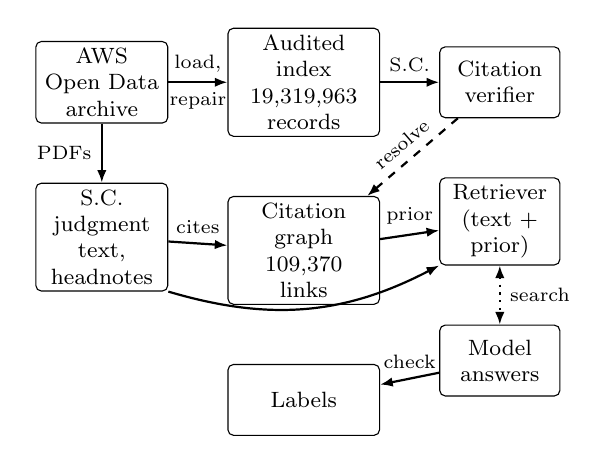
\begin{tikzpicture}[
  box/.style={draw, rounded corners=2pt, align=center, font=\footnotesize, minimum height=0.9cm, inner sep=2.5pt},
  arr/.style={-{Latex[length=1.6mm]}, thick},
  lbl/.style={font=\scriptsize, align=center}]
\node[box, text width=1.5cm] (aws) {AWS Open Data archive};
\node[box, text width=1.75cm, right=0.75cm of aws] (idx) {Audited index\\ \CorpusTotal{}\\ records};
\node[box, text width=1.35cm, right=0.75cm of idx] (ver) {Citation\\ verifier};
\node[box, text width=1.5cm, below=0.75cm of aws] (txt) {S.C. judgment text, headnotes};
\node[box, text width=1.75cm, below=0.75cm of idx] (graph) {Citation graph\\ \GraphEdges{}\\ links};
\node[box, text width=1.35cm, below=0.75cm of ver] (ret) {Retriever\\ (text + prior)};
\node[box, text width=1.35cm, below=0.75cm of ret] (llm) {Model\\ answers};
\node[box, text width=1.75cm, below=0.75cm of graph] (lab) {Labels};
\draw[arr] (aws) -- node[lbl, above] {load,} node[lbl, below] {repair} (idx);
\draw[arr] (idx) -- node[lbl, above] {S.C.} (ver);
\draw[arr] (aws) -- node[lbl, left] {PDFs} (txt);
\draw[arr] (txt) -- node[lbl, above] {cites} (graph);
\draw[arr, dashed] (ver) -- node[lbl, sloped, above] {resolve} (graph);
\draw[arr] (graph) -- node[lbl, above] {prior} (ret);
\draw[arr] (txt.south east) to[bend right=22] (ret.south west);
\draw[arr, {Latex[length=1.6mm]}-{Latex[length=1.6mm]}, dotted] (ret) -- node[lbl, right] {search} (llm);
\draw[arr] (llm) -- node[lbl, above] {check} (lab);
\end{tikzpicture}
\caption{Overview. The archive's metadata is loaded into an audited index; the verifier resolves citations and case names against its Supreme Court part. The text of every Supreme Court judgment yields headnotes and the citations each judgment makes, which the verifier resolves into a citation graph. The retriever searches headnotes by subject and ranks with the graph's citation counts. Model answers are checked by the verifier; in the search conditions the model queries the index or the retriever before answering.}
\label{fig:pipeline}
\end{figure}


\section{Related Work}
\label{sec:related}
\textbf{Legal hallucination.} Dahl et al.\ asked LLMs verifiable questions about United States federal cases and found hallucination rates between 58\% (ChatGPT~4) and 88\% (Llama~2) \cite{dahl2024}. Magesh et al.\ found that commercial retrieval-augmented legal research tools still hallucinate on 17--33\% of queries \cite{magesh2025}. Liu et al.\ collected over 1{,}000 court filings containing fabricated citations and benchmarked automatic detectors on 1{,}300 brief excerpts with injected errors \cite{liu2026checks}. LegalCiteBench evaluates 21 models on citation tasks built from 1{,}000 United States opinions and finds that even the strongest scores below 7/100 on citation retrieval and completion \cite{legalcitebench}; Verma shows that models catch substituted cases far more reliably than wrong pinpoint pages \cite{verma2026}. All of these studies concern United States law.

\textbf{Citation tools.} eyecite extracts and normalises United States legal citations \cite{eyecite}, and CourtListener's citation lookup API matches them against its database to flag invalid ones \cite{courtlistenerapi}. Our verifier plays the same role for the Supreme Court of India, whose citation formats (neutral citations, S.C.R. supplementary volumes) and party-name conventions differ.

\textbf{Citation networks and case retrieval.} Fowler et al.\ built the citation network of all majority opinions of the United States Supreme Court and derived measures of the legal importance of precedents \cite{fowler2007}. For India, Minocha et al.\ studied a citation network of judgments that invoke Articles 264--300 of the Constitution \cite{minocha2015}. Prior-case retrieval asks for the earlier judgments a case should cite. The Indian IL-PCR benchmark takes its relevance judgments from the citations in the judgments themselves \cite{joshi2023ucreat}, as citation recommendation does in general \cite{farber2020}. Retrieval-augmented generation grounds a model's answer in retrieved documents \cite{lewis2020rag}. We build the citation network for the whole reported Supreme Court, use it both as a ranking signal and as relevance labels, and measure what retrieval changes in the authorities that models cite.

\textbf{Agents with citation checks.} Recent legal agents retrieve sources before answering and audit their own citations: L-MARS measures citation faithfulness claim by claim \cite{lmars}, an agentic retrieval system answers 95.3\% of 300 multiple-choice questions from the Korean bar examinations \cite{koreanrag}, Maat grounds competition-law answers in official decisions \cite{maat}, and Parthenon wraps agents in deterministic checks for sources, dates and numbers \cite{parthenon}. A recent survey reviews this line of work \cite{liu2026survey}. Our verifier can serve as such a check for Indian law.

\textbf{Indian legal NLP resources.} ILDC provides 35k Supreme Court judgments for judgment prediction \cite{ildc}, IL-TUR benchmarks Indian legal text understanding \cite{iltur}, and NyayaRAG studies retrieval-augmented judgment prediction \cite{nyayarag}. Juvekar et al.\ evaluate frontier models on Indian legal examinations and name citation discipline as a recurring failure \cite{juvekar2025}, and Hemrajani's survey experiment finds that LLMs frequently fabricate authorities in Indian legal research tasks \cite{hemrajani2025}. Closest to our corpus, open-india-law releases extracted text and embeddings for 12.8 million judgments from the same AWS archive and treats a citation graph as out of scope \cite{openindialaw}. We add a documented audit of the archive's metadata, a citation verifier, an open citation graph of the Supreme Court and a benchmark of how models cite.

\section{An Open Index of Indian Judgments}
\label{sec:corpus}
\subsection{Source and loading}
The AWS Open Data registry hosts two datasets published under CC-BY-4.0 by Dattam Labs: judgments of the Supreme Court from 1950 \cite{awssc} and of 25 High Courts \cite{awshc}, each with structured metadata in Parquet and the judgments as PDFs. We load only the metadata (no text and no PDFs) into one PostgreSQL 17 table, reading the Parquet files directly from S3 (for the large High Court files, only the needed columns). The result holds \CorpusTotal{} records: \CorpusSC{} Supreme Court judgments and \CorpusHC{} High Court judgments and orders from the 25 High Courts (\CorpusCourts{} courts in all), with decision years from \CorpusYearMin{} to \CorpusYearMax. Each record stores a link to the original PDF in the archive, never the PDF itself; the text of the Supreme Court judgments, used in \S\ref{sec:graph}, is extracted separately.

\subsection{Audit and repair}
High Court metadata reaches the archive through two paths. Records from the ``mobile'' path store only a bare file name where a bench-qualified path is needed, so the PDF link cannot be formed. The archive's documentation notes that mobile records may lack a PDF-existence flag and recommends the case number, decision date and order number as the record identity \cite{hcdatasetdoc}, but it does not quantify the problem. Table~\ref{tab:mobile} does. \MobileTotal{} records in four High Courts (\MobilePct{} of the corpus) are affected, \MobileRecentPct{} of them decided in 2024--2026.

The file name is not a usable identity either: \CollideStems{} file names occur in more than one bench of the same court, covering \CollideRows{} records. In \CollideDiffBothPct{} of these the title and the decision date both differ, so the records are different orders. Keying on the file name, as our first load did, silently overwrites at least \CollideLost{} records. The case number (CNR) differs in all of them, so the documented identity is safe.

We repair the mobile records by taking the bench from the S3 key of the metadata file and then reconciling every record against a listing of the archive's actual PDF files. A record is linked only when its file exists. This restores \MobileLinked{} links (\MobileLinkedPct). The remaining \MobileUnrecov{} records have no matching PDF in the archive's file listing; they include all but \MPLinked{} of Madhya Pradesh's \MPMobile{} mobile records. After repair \LinkedPct{} of all records carry a link.

\begin{table}[t]
\caption{High Court records from the archive's mobile path, and the links restored by reconciliation against the archive's file listing.}
\label{tab:mobile}
\centering
\begin{tabular}{lrrr}
\toprule
High Court & Records & Mobile & Linked after repair \\
\midrule
Bombay & 2{,}446{,}330 & 643{,}216 & 537{,}441 (83.6\%) \\
Allahabad & 2{,}300{,}821 & 605{,}598 & 584{,}934 (96.6\%) \\
Madhya Pradesh & 693{,}219 & 42{,}695 & 5 ($<$0.1\%) \\
Himachal Pradesh & 292{,}894 & 7 & 7 (100.0\%) \\
\midrule
All four & 5{,}733{,}264 & 1{,}291{,}516 & 1{,}122{,}387 (86.9\%) \\
\bottomrule
\end{tabular}

\end{table}

\subsection{Validation}
We checked links against the live archive with HTTP HEAD requests. All \RecoveredChecked{} randomly sampled restored links resolve. For \UnresolvedChecked{} randomly sampled unrecoverable records we requested the expected file in the decision-year folder and the two neighbouring years; none exists. For the original, non-mobile links we drew a per-court random sample: all \NonmobileChecked{} resolve, across \NonmobileCourts{} High Courts, as do all \SCLinksChecked{} sampled Supreme Court links. Of \PairsChecked{} randomly sampled file names shared by two benches, all \PairsDiffer{} pairs point to different files (different size and S3 ETag).

\subsection{Supreme Court citation metadata}
Every one of the \CorpusSC{} Supreme Court judgments carries an S.C.R. citation, \SCSupp{} of them (\SCSuppPct) in a supplementary volume (e.g., \texttt{[1995] SUPP.~2 S.C.R.~359}), and \SCwithNeutral{} carry a neutral citation. The Supreme Court launched neutral citations in 2023 in the form \texttt{2023INSC1}: year of pronouncement, \texttt{INSC}, serial number \cite{scneutral}. Three properties of the metadata matter for verification:
\begin{enumerate}
\item The year field of a Supreme Court record is the year of its S.C.R. volume, not of the decision; they differ for \SCYearNe{} judgments (\SCYearNePct). We use the decision date throughout.
\item \SCDupGroups{} neutral citations are attached to more than one record (\SCDupRows{} records), for example a 2018 referral order that carries the neutral citation of the 2020 judgment in the same matter.
\item For each year from 1950 to 2013 except \INSCIncompleteList, the index contains every neutral-citation number from 1 to the year's maximum. This matches how the numbers were issued: for 1950--2013 the Court assigned neutral citations retrospectively to the judgments reported in the S.C.R. \cite{scneutral2}. From 2014 the Court numbers judgments and orders whether or not they are reported, and the index, which holds reported judgments, contains between \INSCCovMin{} and \INSCCovMax{} of each year's numbers. A neutral citation missing from the index is therefore unassigned only for the \INSCCompleteCount{} complete years.
\end{enumerate}

\subsection{Serving}
A small HTTP service exposes keyword search, filters and exact lookups for CNR, neutral and S.C.R. citations. On a laptop (Intel Core i7-13700HX, 32\,GB RAM, NVMe SSD) with default PostgreSQL settings, exact lookups answer in a median of \LatExactMedian{}\,ms over HTTP; keyword queries are slower and depend on phrase frequency (\S\ref{sec:discussion}).

\section{Citation Verifier}
\label{sec:verifier}
The verifier takes a case name, a year and a citation string, as a model produced them, and decides whether they denote a real Supreme Court judgment in the index.

\textbf{Citations.} Neutral citations are parsed with the pattern \emph{year} \texttt{INSC} \emph{number}. S.C.R. citations are parsed in the bracketed official form and the common variants \texttt{(1978) 2 SCR 621} and \texttt{1995 (3) SCR 1}; a citation without a volume number (common for supplementary volumes, e.g.\ \texttt{[1973] Supp.\ S.C.R.~1}) matches any volume of the same series, year and page. Citations to other law reports (SCC, AIR and others) cannot be resolved against the index and are left to the name match.

\textbf{Names.} A case name and a judgment's party names are split into words and initials. Words are lower-cased, stop-words such as \emph{the}, \emph{v.}\ and \emph{ors.}\ are dropped, and abbreviations are expanded (\emph{C.B.I.}, \emph{A.D.M.}, and state codes such as \emph{U.P.}\ when they follow ``of''); single letters written as initials, as in \emph{K.S.\ Puttaswamy}, are kept apart. Each word $t$ has weight $w(t)=\log(N/\mathrm{df}(t))$ over the $N$ Supreme Court judgments \cite{sparckjones}; a word absent from the index gets weight $\log N$. Two words match if they are equal or, for words of five or more letters, if their similarity ratio \cite{difflib} is at least 0.85, which accepts transliteration variants such as \emph{Keshavananda}/\emph{Kesavananda} but not \emph{Patil}/\emph{Patel}. Once a distinctive word (one found in at most 100 judgments) has matched, a rare given name may also match an initial in the judgment's title, as \emph{Shivkant} matches the ``S.'' of ``S.~S.~Shukla''. With $M_a$ and $M_b$ the matched words of the name $a$ and of the judgment $b$, let $p=W(M_a)/W(a)$ and $r=W(M_b)/W(b)$, where $W$ sums word weights. The name score is the harmonic mean of $p$ and $r$, set to zero if $p<0.8$, so that an unmatched given name (\emph{Kavita Devi} against \emph{Ram Kumari Devi}) cannot be outweighed by common words such as \emph{State} or \emph{Uttar Pradesh}, and set to zero if the initials in the cited name do not appear in the judgment's title, either as initials or, after a distinctive match, as the first letters of names the title spells out (\emph{R.D.}\ for \emph{Ramana Dayaram}). Candidates are judgments whose decision year or S.C.R. volume year lies within one year of the stated year.

\textbf{Labels.} With threshold $\tau=0.5$:
\emph{VERIFIED} if some candidate's name score is at least $\tau$ and a neutral or S.C.R. citation, if given, points to that judgment or to one with matching parties;
\emph{WRONG\_CITATION} if the parties match but the citation points elsewhere or nowhere;
\emph{MISATTRIBUTED} if no candidate matches but the citation resolves to a different judgment;
\emph{WRONG\_YEAR} if neither resolves but the name identifies exactly one judgment (or several orders in one matter) elsewhere in the corpus, with a score of at least 0.8 and a word found in at most 15 judgments, i.e.\ a real case cited with the wrong year;
\emph{NOT\_FOUND} otherwise.
VERIFIED establishes that a judgment with those parties exists near that year, not that it supports the proposition for which it was cited.

\textbf{Development.} We developed these rules and thresholds on the T4 answers of three models, reviewing by hand a development sample of 56 decisions and every label that changed between versions of the rules. We then froze the verifier, recording hashes of its code, before running T5, scoring, and drawing the held-out audit reported in \S\ref{sec:audit}. One OCR error in the title of a benchmark judgment (\emph{T.M.A.\ Pal} for \emph{Pai}) is corrected when the index is loaded.

\section{Judgment Text and Citation Graph}
\label{sec:graph}
\subsection{Text and headnotes}
We downloaded the PDF of every Supreme Court judgment in the archive and extracted its text layer with PyMuPDF. The reports are scanned pages with an embedded OCR layer, so no further OCR is needed; we keep only the text. \GraphTextOK{} of the \CorpusSC{} judgments were extracted; for \GraphTextFail{} the archive returned an error or an HTML page instead of the PDF. Every judgment in the S.C.R. opens with the reporter's headnote: the parties, date and bench, then a summary of the questions decided and the holdings, then the judgment proper, usually introduced by a jurisdiction line such as ``CIVIL APPELLATE JURISDICTION''. We cut the headnote at that line, keep at most 3{,}000 characters, and remove running page heads and the margin letters A--H of the printed report.

\subsection{Extracting and resolving citations}
We find every reporter citation in the text: S.C.R. and neutral citations, SCC citations, and AIR citations of the Supreme Court (AIR citations of other courts are discarded). Each distinct pair of citing judgment and citation is resolved in three tiers:
\begin{enumerate}
\item \emph{Number}: an S.C.R. or neutral citation is looked up exactly in the index.
\item \emph{Parallel number}: an SCC or AIR citation written directly beside an S.C.R. or neutral citation, as in \texttt{(2012) 1 SCC 40 : [2011] 13 SCR 309}, takes that number's judgment.
\item \emph{Name}: otherwise the case name written before the citation and the citation's year go through the frozen verifier of \S\ref{sec:verifier}, and the pair is resolved only if exactly one judgment matches.
\end{enumerate}
If a number and the case name beside it point to different judgments, the pair is dropped. A citation of the judgment itself (its own report) is ignored. We developed the extractor on a pilot sample of \PilotN{} judgments and then ran it once over the whole corpus; the manual check in \S\ref{sec:graphres} uses only judgments outside the pilot.

\subsection{Size and accuracy}
\label{sec:graphres}
Across the \GraphTextOK{} judgments the extractor found \GraphUnits{} distinct pairs of a citing judgment and a reporter citation of another judgment. \GraphResolved{} of them (\GraphResolvedPct) were resolved: \GraphExact{} by number, \GraphParallel{} through a parallel number and \GraphName{} by case name and year. \GraphConflict{} pairs whose number and name disagreed were dropped. The resolved pairs form \GraphEdges{} distinct links between \GraphCiting{} citing and \GraphCited{} cited judgments, so \GraphCitedPct{} of the Supreme Court's reported judgments are cited by at least one later reported judgment. Resolution depends on the era of the citing judgment (Table~\ref{tab:graph}). Until the 1980s judgments cite mostly the S.C.R. and are resolved by number. From the 1990s the commercial SCC is the most cited report. Parallel S.C.R. citations, which make recent judgments easy to resolve, become common only in the 2010s, so the 2000s are the hardest decade.

\begin{table}[t]
\caption{Citations of other reported judgments, by decade of the citing judgment, and how they were resolved.}
\label{tab:graph}
\centering
\footnotesize
\setlength{\tabcolsep}{4pt}
\begin{tabular}{lrrrrr}
\toprule
Citing & Citations & Resolved & \multicolumn{3}{c}{Resolved by} \\
\cmidrule(lr){4-6}
decade & & (\%) & Number & Parallel & Name \\
\midrule
1950s & 953 & 87.6 & 821 & 0 & 14 \\
1960s & 3{,}259 & 84.0 & 2{,}669 & 6 & 63 \\
1970s & 5{,}001 & 75.9 & 3{,}561 & 18 & 219 \\
1980s & 6{,}467 & 77.5 & 4{,}160 & 43 & 806 \\
1990s & 15{,}667 & 63.8 & 4{,}958 & 361 & 4{,}676 \\
2000s & 34{,}810 & 55.0 & 2{,}957 & 375 & 15{,}830 \\
2010s & 70{,}340 & 78.5 & 23{,}027 & 17{,}174 & 15{,}026 \\
2020s & 67{,}418 & 84.0 & 26{,}370 & 22{,}036 & 8{,}212 \\
\bottomrule
\end{tabular}

\end{table}

\textbf{Accuracy.} Where a citation carries an S.C.R. or neutral number and the case name beside it can also be resolved, the name and year alone reach the same record as the number in \GraphNameSamePct{} of \GraphNamePrecN{} cases. In another \GraphNameLoosePct{} they reach a different record with matching parties (for example another order in the same case), and in \GraphNameWrongPct{} a record with different parties. This is a label-free estimate of the precision of name-only links. Only \GraphLater{} links (\GraphLaterPct) point to a judgment decided after the citing one, which is impossible. In a sample of them the causes were wrong decision dates in the metadata, page numbers of a neighbouring judgment in the same report volume, and truncated generic names (\emph{Others v.\ The State of Assam}) matched to the wrong judgment. Because name matching is restricted to the cited year, most wrong links cannot point forward, so this check is a sanity check, not an error bound. We also checked by hand \GraphCheckN{} randomly drawn name-only links from judgments outside the pilot, against the citation context and the index record: all \GraphCheckOK{} were correct, including names misspelt in the citing text, such as \emph{A.N.\ Shehgal} for \emph{A.N.\ Sehgal}. Of \UnresN{} randomly drawn SCC and AIR citations that stayed unresolved, \UnresNotIndex{} cite judgments that are not in the index at all, because they were reported in the SCC or AIR but not in the S.C.R. The other \UnresInIndex{} could have been resolved: \UnresExtraction{} were lost to OCR errors or truncated names in the citing text, \UnresSource{} to errors in the source (a wrong year in the citation, a misspelt index title), \UnresAmbig{} to names shared by several judgments, and \UnresVerifier{} to limitations of the frozen name parser.

\textbf{Face validity.} The most cited judgments are \emph{Maneka Gandhi v.\ Union of India} (\GraphTopOneN{} citing judgments), \emph{Kesavananda Bharati} (\GraphTopTwoN), \emph{Sharad Birdhi Chand Sarda v.\ State of Maharashtra} (\GraphTopThreeN), \emph{Ramana Dayaram Shetty v.\ International Airport Authority} (\GraphTopFourN) and \emph{Shivaji Sahebrao Bobade v.\ State of Maharashtra} (\GraphTopFiveN): leading authorities on personal liberty, the basic structure, circumstantial evidence, State action and criminal appeals. Of the \GraphLandmarkN{} landmark judgments that we chose by hand for the benchmark before the graph existed, \GraphLandmarkCited{} are cited at least once, and their median in-degree is higher than that of \GraphLandmarkPct\% of all judgments.


\section{Finding Authorities by Subject}
\label{sec:retrieval}
\subsection{Retrievers}
We index the title and headnote of every judgment in two ways. \emph{BM25} \cite{robertson2009} scores unigrams and bigrams (English stop words removed). \emph{Dense} retrieval embeds each headnote with the open multilingual model bge-m3 \cite{chen2024m3}, run locally, and scores by cosine similarity with the embedded query. The \emph{hybrid} retriever takes the union of the top 300 judgments of each and adds their scores after normalising each to zero mean and unit variance over the candidates. A \emph{citation prior} adds the normalised $\log(1+c)$, where $c$ is the number of judgments in the graph that cite the candidate. We use the raw count; recursive measures such as PageRank \cite{page1999} are an alternative that we did not test. Every combination is a weighted sum of these three scores; the weights are chosen on a development split and never on the evaluation data.

\subsection{Evaluation without human labels}
The graph supplies relevance judgments without annotation: the judgments a decision cites are the authorities its bench considered, the standard setting of citation recommendation \cite{farber2020} and of Indian prior-case retrieval \cite{joshi2023ucreat}. For each held-out judgment that cites at least \RecMinTargets{} earlier judgments, the query is its headnote with every reporter citation, every ``X v.\ Y'' case name and every ``\ldots's case'' reference removed, so the query states the legal issues without naming the precedents. The targets are the judgments it cites. Only judgments decided before it are candidates, and the citation prior counts only citations made before it, so no information from the future is used. We choose weights on \RecNDev{} development judgments and report recall@10, recall@50, the share of queries with at least one target in the top 10 (hit@10) and mean reciprocal rank on \RecNTest{} other test judgments, with bootstrap 95\% intervals. We also score the 40 T4 questions against their reference judgments, with the weights from the development split.

\subsection{Results}
\label{sec:retres}
\textbf{Citation recommendation.} \RecPool{} judgments cite at least \RecMinTargets{} earlier judgments that the graph resolves. On the \RecNTest{} test judgments, which cite \RecMeanTargets{} of them on average, the hybrid retriever with the citation prior places \RecHybridPriorRTenPct{} of the cited judgments in its top 10, and at least one of them for \RecHybridPriorHitTen{} of the queries (Table~\ref{tab:recommend}). The prior helps every retriever. On the same queries it raises the recall@10 of the hybrid retriever by \RecDiffPrior{} (paired bootstrap 95\% CI \RecDiffPriorCI; better on \RecDiffPriorBetter{} queries, worse on \RecDiffPriorWorse), a relative gain of \RecPriorRelGain. Popularity alone is useless (\RecPopRTen). The prior only reorders judgments that already match the subject, and among those, the ones the Court has cited often are more likely to be cited again. The query scrubbing leaves some names behind: \RecLeakStrictPct{} of the cited judgments share a rare title word (one found in at most \RecLeakRareDF{} titles) with the query. Scoring only the other targets changes little (\RecHybridPriorRTenUnleaked{} with the prior, \RecHybridRTenUnleaked{} without).

\begin{table}[t]
\caption{Citation recommendation on \RecNTest{} held-out judgments: given the headnote without citations and case names, retrieve the earlier judgments it cites. R@$k$ = share of cited judgments in the top $k$; Hit@10 = share of queries with at least one in the top 10; MRR = mean reciprocal rank of the first. Weights chosen on \RecNDev{} other judgments.}
\label{tab:recommend}
\centering
\footnotesize
\setlength{\tabcolsep}{4pt}
\begin{tabular}{lrrrr}
\toprule
Method & R@10 & R@50 & Hit@10 & MRR \\
\midrule
Most cited so far & 0.013 & 0.039 & 0.111 & 0.056 \\
BM25 & 0.151 & 0.321 & 0.662 & 0.390 \\
Dense (bge-m3) & 0.136 & 0.286 & 0.614 & 0.362 \\
BM25 + dense & 0.167 & 0.345 & 0.689 & 0.420 \\
BM25 + prior & 0.182 & 0.381 & 0.740 & 0.455 \\
Dense + prior & 0.159 & 0.323 & 0.686 & 0.426 \\
BM25 + dense + prior & 0.204 & 0.399 & 0.774 & 0.496 \\
\bottomrule
\end{tabular}

\end{table}

\textbf{The 40 legal questions.} Searched with the question text, the hybrid retriever with the prior returns a judgment that decided the question among its top three results for \QHybridPriorHitThree{} of the \NumTopics{} questions, and among its top ten for \QHybridPriorHitTen{} (Table~\ref{tab:questions}). No model named such a judgment from memory for more than \RefClosedLlama{} questions. Every judgment the retriever returns exists, with its correct citations, by construction. The questions were written around landmark judgments, which are cited often, so this set favours the prior. The recommendation experiment has no such bias.

\begin{table}[t]
\caption{Retrieval for the \NumTopics{} T4 questions: questions whose top-$k$ results contain a reference judgment, and the share of reference judgments in the top 10 (R@10). Weights from the recommendation development split.}
\label{tab:questions}
\centering
\footnotesize
\setlength{\tabcolsep}{4pt}
\begin{tabular}{lrrrr}
\toprule
Retriever & Top 3 & Top 5 & Top 10 & R@10 \\
\midrule
Most cited & 2 & 2 & 2 & 0.04 \\
BM25 & 25 & 28 & 30 & 0.63 \\
Dense & 29 & 31 & 35 & 0.76 \\
BM25 + dense & 28 & 30 & 36 & 0.77 \\
BM25 + dense + prior & 33 & 35 & 37 & 0.84 \\
\bottomrule
\end{tabular}

\end{table}


\section{How Language Models Cite: Setup}
\label{sec:setup}
\subsection{Items}
The benchmark uses \NumJudgments{} Supreme Court judgments: \NumLandmark{} landmark judgments that we identified by name and confirmed individually in the index, and \NumRandom{} judgments sampled at random (seeded) across eight periods from 1950 to 2023. Landmark candidates were dropped when the index record was ambiguous or erroneous (e.g., a shared neutral citation). All benchmark judgments have a unique neutral citation whose year equals the decision year.
\begin{itemize}
\item \textbf{T1, real citation $\rightarrow$ case} (\NumTOne{} items): each judgment is asked for once by its S.C.R. citation and once by its neutral citation: \emph{Which judgment of the Supreme Court of India is reported as~\ldots?} The answer is correct if the named parties match the true judgment (name score $\ge\tau$).
\item \textbf{T2, fabricated citation} (\NumTTwo{} items): the same question for citations that cannot exist: 30 neutral citations in complete years with a number between $2m+100$ and $3m+100$, where $m$ is the year's last issued number, and 30 S.C.R. citations to a regular volume at least three above the year's last. The correct response is to decline.
\item \textbf{T3, case $\rightarrow$ citation} (\NumTThree{} items): given the parties and decision date, the model gives the S.C.R. and neutral citations; each is scored by exact match (with the volume rule above).
\item \textbf{T4, authorities for a question} (\NumTopics{} items): the model lists up to three Supreme Court judgments that are leading authorities on a legal question (e.g., whether the right to privacy is a fundamental right), each with year and citation; every case is labelled by the verifier.
\item \textbf{T5, revision after feedback}: for each T4 answer with an unverified case, the model is told which cases the index could not confirm and asked to revise its list.
\end{itemize}
For T4 we also record reference answers: for each question, the Supreme Court judgments that decided it, one to four per question (\NumRefJudgments{} index records, since a matter decided in several orders contributes each order), including earlier decisions later overruled, such as \emph{Suresh Kumar Koushal} for Section~377. We compiled them from the questions after the closed-book runs and before the search runs (\S\ref{sec:searchsetup}), and recorded their hash. A question is answered with a reference judgment if one of the listed cases matches it under the verifier's name and year rules. This is a lower bound on relevance, since the models also cite other pertinent judgments.

\subsection{Models and inference}
We evaluate open-weight models that run on an 8\,GB laptop GPU (NVIDIA RTX 4060) through Ollama \cite{ollama}, all in 4-bit (Q4\_K\_M) quantisation (Table~\ref{tab:models}). Every request uses the same system prompt, which asks the model to state only facts it is confident about and to say when it does not know; temperature~0; a fixed seed; and a JSON schema that constrains the output format, so answers can be parsed without heuristics. Thinking is disabled for the Qwen3 model; as an ablation we also run it with thinking enabled on T1, T2 and T4, allowing 3{,}000 additional output tokens for the reasoning and an 8{,}192-token context.

\begin{table}[t]
\caption{Models evaluated (Ollama builds, 4-bit Q4\_K\_M).}
\label{tab:models}
\centering
\footnotesize
\setlength{\tabcolsep}{4pt}
\begin{tabular}{llrl}
\toprule
Model & Ollama tag & Params & Digest \\
\midrule
Llama 3.1 8B \cite{llama3} & \texttt{llama3.1:8b} & 8.0B & \texttt{46e0c10c} \\
Qwen3 8B \cite{qwen3} & \texttt{qwen3:8b} & 8.2B & \texttt{500a1f06} \\
Qwen3 8B think \cite{qwen3} & \texttt{qwen3:8b} & 8.2B & \texttt{500a1f06} \\
Gemma 3 4B \cite{gemma3} & \texttt{gemma3:4b} & 4.3B & \texttt{a2af6cc3} \\
Qwen2.5-VL 7B \cite{qwen25vl} & \texttt{qwen2.5vl:7b} & 8.3B & \texttt{5ced39df} \\
\bottomrule
\end{tabular}

\end{table}

\subsection{Search conditions}
\label{sec:searchsetup}
In a \emph{name search} condition the models answer the same T1--T4 items with access to the index metadata. The Supreme Court records hold party names, dates and citations but no text, so this search cannot retrieve judgments by subject: it can confirm a judgment the model recalls and supply its citations. The model has two tools. \emph{Search} returns the \SearchK{} judgments whose party names best match the query, ranked by the IDF-weighted name score of \S\ref{sec:verifier} over judgments that share one of the query's three rarest words or a spelling variant of it. \emph{Lookup} returns the judgment with a given neutral or S.C.R. citation, or reports that the index has none. The task prompt is followed by a description of the tools, including what the index holds. The model replies with one action at a time in JSON, receives each result as the next message, and after at most \SearchMaxActions{} actions is asked for its final answer in the task's own schema, which is scored exactly like the closed-book answer. We use this JSON protocol rather than native tool calling because Gemma~3 has none in Ollama. The context is 8{,}192 tokens; all other settings are unchanged. We tried the protocol on four items outside the benchmark, froze it with the reference answers by recording hashes, and then ran it once.

In two \emph{topic search} conditions we repeat T4 with the retriever of \S\ref{sec:retrieval} as the search tool. The protocol is unchanged, but \emph{search} now matches the title and headnote, so the model can search by subject, and each result shows the parties, date, citations and the first 280 characters of the headnote. We use the hybrid retriever, once without and once with the citation prior (weights from the recommendation development split). We checked the protocol on one question outside the benchmark and froze the retrieval code by hash before these runs.

\subsection{Metrics}
For T1 and T2 we report the share of items answered correctly, answered wrongly, and declined; invalid outputs (e.g., a degenerate repetition that hits the length limit) are counted separately. For T4 and T5 we report the share of cited cases in each verifier label, and the number of questions whose list includes a reference judgment. Where we give 95\% intervals they are Wilson intervals \cite{wilson}; for T4 they treat cited cases as independent, although cases cited for the same question are related, so they understate the uncertainty.

\section{How Language Models Cite: Results}
\label{sec:results}

\subsection{Identifying citations (T1, T2)}
Table~\ref{tab:t1t2} shows two opposite behaviours. Llama~3.1 and Gemma~3 answered almost every question and were almost always wrong. Llama identified \TOneCorrectLlama{} of the \TOneN{} real citations (\emph{Kesavananda Bharati}, by its S.C.R. citation); Gemma identified none. Both named a judgment for nearly every fabricated citation: \TTwoNamedLlama{} of 60 for Llama (\TTwoNamedPctLlama, 95\% CI \TTwoNamedCILlama; one output was invalid) and \TTwoNamedGemma{} of 60 for Gemma (\TTwoNamedPctGemma, 95\% CI \TTwoNamedCIGemma). Their wrong answers were not near misses: the closest any wrong T1 answer came to the true judgment was a name score of \MaxWrongLenientLlama{} (Llama) and \MaxWrongLenientGemma{} (Gemma), well below the match threshold of 0.5. The answers also repeated: across T1 and T2, Llama gave \emph{\TopAnswerLlama} as the answer \TopAnswerCountLlama{} times, and Gemma gave \emph{\TopAnswerGemma} \TopAnswerCountGemma{} times. The two Qwen models took the opposite course and declined all 262 questions. Under our system prompt, declining is the correct response to T2, but it forfeits T1 entirely. With thinking disabled, no model identified more than \BestTOneCorrect{} of the \TOneN{} real citations.

\begin{table}[t]
\caption{Identifying a judgment from its citation. T1: \NumTOne{} real citations (\NumJudgments{} judgments, each by S.C.R. and neutral citation). T2: \NumTTwo{} citations that cannot exist. Corr.\ = named the right judgment; Named = named any judgment for a fabricated citation; Decl.\ = declined; Inv.\ = invalid output.}
\label{tab:t1t2}
\centering
\footnotesize
\setlength{\tabcolsep}{3pt}
\begin{tabular}{lrrrrrrr}
\toprule
& \multicolumn{4}{c}{T1: real citation (\%)} & \multicolumn{3}{c}{T2: fabricated (\%)} \\
\cmidrule(lr){2-5}\cmidrule(lr){6-8}
Model & Corr. & Wrong & Decl. & Inv. & Named & Decl. & Inv. \\
\midrule
Llama 3.1 8B & 0.5 & 99.0 & 0.0 & 0.5 & 98.3 & 0.0 & 1.7 \\
Qwen3 8B & 0.0 & 0.0 & 100.0 & 0.0 & 0.0 & 100.0 & 0.0 \\
Qwen3 8B think & 1.0 & 14.4 & 83.2 & 1.5 & 10.0 & 88.3 & 1.7 \\
Gemma 3 4B & 0.0 & 100.0 & 0.0 & 0.0 & 100.0 & 0.0 & 0.0 \\
Qwen2.5-VL 7B & 0.0 & 0.0 & 100.0 & 0.0 & 0.0 & 100.0 & 0.0 \\
\bottomrule
\end{tabular}

\end{table}

\subsection{Supplying citations (T3)}
When given the parties and the date of a judgment and asked for its citations, the two Qwen models, which had declined every T1 question, supplied a neutral citation for most judgments, and almost all were wrong (Table~\ref{tab:t3}). Across the four models only \TThreeCorrectAll{} of the \TThreeAskedAll{} requested citations were correct. Qwen2.5-VL returned a neutral citation for \TThreeNeutralWrongQwenVL{} of \NumTThree{} judgments and none was correct; \TThreeUnassignedQwenVL{} of them carry a number above the year's last issued neutral citation in a year the index covers completely, so they cannot exist. Qwen3 returned wrong neutral citations for \TThreeNeutralWrongQwen{} judgments, \TThreeNeutralOtherJudgmentQwen{} of which belong to other judgments, and wrong S.C.R. citations for \TThreeScrWrongQwen{}, \TThreeScrNoJudgmentQwen{} of which point to a page where no reported judgment begins. Llama answered the request for a neutral citation with an AIR citation \TThreeNeutralOtherFormatLlama{} times.

\begin{table}[t]
\caption{Supplying the citations of \NumTThree{} known judgments, given parties and decision date. Corr.\ = exact match; Wrong = any other non-empty answer; Empty = no citation given.}
\label{tab:t3}
\centering
\setlength{\tabcolsep}{4pt}
\begin{tabular}{lrrrrrr}
\toprule
& \multicolumn{3}{c}{S.C.R. citation (\%)} & \multicolumn{3}{c}{Neutral citation (\%)} \\
\cmidrule(lr){2-4}\cmidrule(lr){5-7}
Model & Corr. & Wrong & Empty & Corr. & Wrong & Empty \\
\midrule
Llama 3.1 8B & 2.0 & 96.0 & 2.0 & 0.0 & 98.0 & 2.0 \\
Qwen3 8B & 0.0 & 83.2 & 16.8 & 1.0 & 80.2 & 18.8 \\
Qwen3 8B think & -- & -- & -- & -- & -- & -- \\
Gemma 3 4B & 0.0 & 100.0 & 0.0 & 0.0 & 100.0 & 0.0 \\
Qwen2.5-VL 7B & 0.0 & 11.9 & 88.1 & 0.0 & 90.1 & 9.9 \\
\bottomrule
\end{tabular}

\end{table}

\subsection{Authorities for legal questions (T4)}
Asked for up to three leading Supreme Court authorities on each of \NumTopics{} questions, the models named between \TFourCasesMin{} and \TFourCasesMax{} cases each, counting a case repeated within one answer once (Table~\ref{tab:t4}). Only \TFourVerifiedRange{} of these could be matched to a Supreme Court judgment with the named parties within a year of the stated date; between \TFourNFMinPct{} (\TFourNFMinModel) and \TFourNFMaxPct{} (\TFourNFMaxModel) were NOT\_FOUND. The models cited almost exclusively the commercial SCC and AIR reports and SCC OnLine, which the index cannot resolve, so these labels rest on the party names and year. Only Qwen2.5-VL used the S.C.R. form to any extent (\TFourReporterCitesQwenVL{} citations, \TFourReporterCitePctQwenVL{} of its total). All \TFourReporterResolvedMisQwenVL{} of these that resolved in the index pointed to a different judgment (MISATTRIBUTED): for example, it attributed \texttt{1970 (2) SCR 1}, which is \emph{Sitabai v.\ Ram Chandra}, to an invented \emph{State of Maharashtra v.\ Keshav Bapuji Patil}. WRONG\_YEAR cases are real judgments cited with a wrong year, such as \emph{R.\ Rajagopal v.\ State of Tamil Nadu} (1994) cited as 1969 and 1985.

\begin{table}[t]
\caption{T4: every case cited for \NumTopics{} legal questions, by verifier label. Ver.\ = VERIFIED (with Wilson 95\% interval), W.Yr.\ = WRONG\_YEAR, W.Cit.\ = WRONG\_CITATION, Misatt.\ = MISATTRIBUTED, N.F.\ = NOT\_FOUND.}
\label{tab:t4}
\centering
\footnotesize
\setlength{\tabcolsep}{3.5pt}
\begin{tabular}{lrrrrrrr}
\toprule
& & \multicolumn{6}{c}{Share of cited cases (\%)} \\
\cmidrule(lr){3-8}
Model & Cases & Ver. & 95\% CI & W.Yr. & W.Cit. & Misatt. & N.F. \\
\midrule
Llama 3.1 8B & 114 & 61.4 & 52--70 & 1.8 & 0.0 & 0.0 & 36.8 \\
Qwen3 8B & 117 & 50.4 & 42--59 & 7.7 & 0.0 & 0.0 & 41.9 \\
Qwen3 8B think & 94 & 35.1 & 26--45 & 4.3 & 0.0 & 0.0 & 60.6 \\
Gemma 3 4B & 117 & 23.9 & 17--32 & 6.8 & 0.0 & 0.0 & 69.2 \\
Qwen2.5-VL 7B & 102 & 22.5 & 16--32 & 0.0 & 0.0 & 11.8 & 65.7 \\
\bottomrule
\end{tabular}

\end{table}

\subsection{Verifier accuracy}
\label{sec:audit}
We built the verifier on a development sample of T4 answers and then froze it. To measure it we drew a fresh, stratified random sample of \AuditN{} T4 decisions from the four models, excluding every case on the development sheet, and judged each by hand against the index and our knowledge of the case law. The verifier was right in \AuditCorrect{} of \AuditN{} (\AuditPct). \AuditVerCorrect{} of \AuditVerN{} VERIFIED labels were correct; the error matched \emph{Narendra Kumar v.\ Union of India} to \emph{State Bank of India v.\ Narendra Kumar Pandey}. \AuditNFCorrect{} of \AuditNFN{} NOT\_FOUND labels were correct; both misses were real judgments whose titles contain OCR errors in the source (\emph{Machhi Singh} spelled ``Machhl'', \emph{Baliya} spelled ``Baliay''). All \AuditWYN{} WRONG\_YEAR and \AuditMisN{} MISATTRIBUTED labels were correct.

The audit also shows what NOT\_FOUND means. Of the \AuditNFN{} audited cases, \AuditNFFab{} named parties that match no Supreme Court judgment in any year, \AuditNFGeneric{} used names so common (\emph{Rajesh Kumar v.\ State of Bihar}) that same-named judgments exist only in other years, \AuditNFMisdated{} was a real judgment cited with both a wrong year and an altered name, \AuditNFNotJudgment{} was not a judgment at all (a committee report), and \AuditNFMiss{} were the verifier misses above.

\subsection{Revision after verifier feedback (T5)}
For the \TFiveQAll{} T4 answers that contained at least one unverified case, we told the model what the check had found for each case (for example, that no Supreme Court judgment with those parties exists near the stated year) and asked it to revise its list. Table~\ref{tab:t5} shows the result. The models dropped the flagged cases: across the four models the number of NOT\_FOUND cases fell from \TFiveNFBeforeAll{} to \TFiveNFAfterAll{}, and the share of verified cases rose for every model. The gain came entirely from removal. \TFiveRepeatedAll{} of the \TFiveCasesAfterAll{} cases in the revised lists were repeated from the first answers; only \TFiveNewCaseModels{} named new cases (\TFiveNewCasesAll{} in all), and none of them could be verified. The number of verified cases fell slightly, from \TFiveVerBeforeAll{} to \TFiveVerAfterAll{}. Qwen3 returned an empty list for \TFiveEmptyAfterQwen{} questions, and Qwen2.5-VL's revised lists still contained \TFiveKeptNFQwenVL{} cases the index could not find, all repeated from its first answers. Feedback from an existence check thus makes an answer shorter and safer, but not more complete.

\begin{table}[t]
\caption{T5: the T4 answers that contained an unverified case (Q), before and after the model revised them with the verifier's feedback.}
\label{tab:t5}
\centering
\footnotesize
\setlength{\tabcolsep}{3.5pt}
\begin{tabular}{lrrrrrrr}
\toprule
& & \multicolumn{2}{c}{Cases} & \multicolumn{2}{c}{Verified (\%)} & \multicolumn{2}{c}{Not found} \\
\cmidrule(lr){3-4}\cmidrule(lr){5-6}\cmidrule(lr){7-8}
Model & Q & Before & After & Before & After & Before & After \\
\midrule
Llama 3.1 8B & 30 & 87 & 48 & 49.4 & 87.5 & 42 & 4 \\
Qwen3 8B & 29 & 84 & 27 & 30.9 & 92.6 & 49 & 1 \\
Gemma 3 4B & 37 & 111 & 40 & 19.8 & 52.5 & 81 & 16 \\
Qwen2.5-VL 7B & 35 & 87 & 39 & 9.2 & 20.5 & 67 & 31 \\
\bottomrule
\end{tabular}

\end{table}

\subsection{Effect of reasoning}
With thinking enabled, Qwen3 wrote a median of \ThinkMedianChars{} characters of reasoning per item and took a median of \ThinkMedianSec{}\,s instead of \NoThinkMedianSec{}\,s (Table~\ref{tab:t1t2}, row ``Qwen3 8B think''; T3 was not run). It stopped declining every question, and the additional answers were mostly wrong. On T1 it identified \ThinkTOneCorrect{} real citations correctly and \ThinkTOneWrong{} wrongly, declining \ThinkTOneDecl{}; on T2 it named a judgment for \ThinkTTwoNamed{} of the 60 fabricated citations (\TTwoNamedPctQwenThink, 95\% CI \TTwoNamedCIQwenThink), sometimes a famous one: it identified the non-existent \texttt{[1992] 7 S.C.R.~142} as \emph{Indra Sawhney v.\ Union of India} and \texttt{[1997] 7 S.C.R.~501} as \emph{Vishaka v.\ Rajasthan}. On T4 the share of verified cases fell from \NoThinkTFourVerPct{} to \ThinkTFourVerPct{} and the share of NOT\_FOUND cases rose from \NoThinkTFourNFPct{} to \ThinkTFourNFPct{}; \ThinkTFourInvalid{} of the 40 answers were invalid because the reasoning exhausted the token budget (\ThinkTruncated{} items in all). At this scale, reasoning made the model more willing to answer without making it more accurate.


\subsection{Searching by name}
\label{sec:search}
With access to the index the citation tasks became easy for most models (Table~\ref{tab:searchcit}). The models identified between \SearchTOneCorrectMin{} and \SearchTOneCorrectMax{} of the \TOneN{} real citations, against at most \BestTOneCorrect{} without search, and three of them supplied the correct S.C.R. and neutral citations for nearly every T3 judgment. Llama and Qwen3 looked up the given citation in every T1 and T2 item. After an empty lookup Llama named a judgment for only \SearchTTwoNamedLlama{} fabricated citation, against \TTwoNamedLlama{} without search. Two weaknesses remain. Gemma looked up the given citation in only \SearchTOneLookedGemma{} of the \TOneN{} T1 items. In the others it searched for a case name it had guessed, never saw the right judgment, and answered from those results or declined; it gave \SearchTOneWrongGemma{} wrong answers in all. For \SearchTTwoNamedGemma{} of the 60 fabricated citations it still named a judgment, \SearchTTwoNamedRealGemma{} of them real judgments that its own searches for invented names had returned. Qwen2.5-VL declined \SearchTOneDeclQwenVL{} T1 items although the lookup had returned the right judgment. Some answers scored wrong do name the right judgment, with a small copying error that the strict name matcher rejects (\emph{Ircc} for \emph{IRRC}, \emph{Simplicity} for \emph{Simplex}, or a title copied with an empty respondent, ``\ldots\ v.'', whose ``v'' the frozen parser reads as an initial). This applies to \SearchTOneNearLlama{} of Llama's \SearchTOneWrongLlama{} and \SearchTOneNearQwen{} of Qwen3's \SearchTOneWrongQwen{} wrong T1 answers. We count them as wrong, as scored.

\begin{table}[t]
\caption{Citation tasks with search and lookup (compare Tables~\ref{tab:t1t2} and~\ref{tab:t3}). T1: \NumTOne{} real citations; T2: \NumTTwo{} fabricated citations; T3: share of the \NumTThree{} judgments whose S.C.R. or neutral citation was supplied exactly.}
\label{tab:searchcit}
\centering
\footnotesize
\setlength{\tabcolsep}{3pt}
\begin{tabular}{lrrrrrrr}
\toprule
& \multicolumn{3}{c}{T1 (\%)} & \multicolumn{2}{c}{T2 (\%)} & \multicolumn{2}{c}{T3 corr.\ (\%)} \\
\cmidrule(lr){2-4}\cmidrule(lr){5-6}\cmidrule(lr){7-8}
Model & Corr. & Wrong & Decl. & Named & Decl. & S.C.R. & Neutr. \\
\midrule
Llama 3.1 8B & 99.0 & 1.0 & 0.0 & 1.7 & 98.3 & 73.3 & 73.3 \\
Qwen3 8B & 97.5 & 2.5 & 0.0 & 0.0 & 100.0 & 100.0 & 100.0 \\
Gemma 3 4B & 49.5 & 49.0 & 1.5 & 51.7 & 48.3 & 99.0 & 99.0 \\
Qwen2.5-VL 7B & 86.6 & 0.0 & 13.4 & 0.0 & 100.0 & 100.0 & 100.0 \\
\bottomrule
\end{tabular}

\end{table}

For legal questions the effect differs (Table~\ref{tab:t4conds}, name search). Name search almost eliminated cases that the index cannot find: across the four models, NOT\_FOUND cases fell from \NFClosedAll{} to \NFSearchAll{}, and verified cases rose from \VerClosedAll{} to \VerSearchAll{}. But fewer answers contained a judgment that decided the question: \RefSearchAll{} of the \RefQuestionsAll{} model--question pairs, against \RefClosedAll{} without search. Pair by pair, \RefLostAll{} lost their reference judgment and \RefGainedAll{} gained one. Because the four models answer the same questions, the pairs are not independent; counting each question once, \SignClosedNameWorse{} questions were answered by fewer models with name search and \SignClosedNameBetter{} by more (exact sign test, $p$~\SignClosedNameP).

The cause is how the models searched. The tool description stated that the index holds no subject matter, yet Llama and Qwen2.5-VL mostly searched with the words of the question: \SearchTopicQLlama{} of Llama's \SearchSearchesLlama{} searches and \SearchTopicQQwenVL{} of Qwen2.5-VL's \SearchSearchesQwenVL{} consisted mainly of the question's own words. They then listed the judgments whose party names happened to contain those words. On whether ``procedure established by law'' must be fair, just and reasonable, Llama had cited \emph{Maneka Gandhi} without search; with search it listed \emph{Fair Air Engineers v.\ N.K.\ Modi} and \emph{Just Society v.\ Union of India}. Qwen2.5-VL listed \emph{State of U.P.\ v.\ U.P.\ State Law Officers Association} and \emph{Bajaj Auto v.\ Company Law Board}. These judgments exist, so the verifier labels them VERIFIED. Yet none of the \SearchTopicCasesAll{} listed judgments that came only from such searches is a reference judgment.

Qwen3 searched by party names (only \SearchTopicQQwen{} of its \SearchSearchesQwen{} searches consisted mainly of the question's words) and kept nearly all its reference hits (\RefClosedQwen{} questions without search, \RefSearchQwen{} with): search confirmed the judgments it recalled but added none it did not. Gemma also searched by names, but paired the citations it found with names from memory, producing \SearchTFourMisGemma{} MISATTRIBUTED cases, such as \emph{Jacob Mathew v.\ State of Kerala} with the citation of \emph{Jacob Mathew v.\ State of Punjab}. Gemma and Qwen2.5-VL often wrote their whole answer into the \emph{answer} action (\SearchTFourInvalidActionGemma{} and \SearchTFourInvalidActionQwenVL{} of 40 T4 episodes), which was cut at the length limit; they were then asked for the final answer as in every other episode.

\begin{table*}[t]
\caption{T4 under five conditions: from memory, after verifier feedback (T5 answers where revised, T4 otherwise), with name search over the index metadata, and with topic search over headnotes without and with the citation prior. Ref.\ = questions (of \NumTopics) whose list includes a judgment that decided the question; N.F.\ = listed cases the verifier could not find.}
\label{tab:t4conds}
\centering
\footnotesize
\setlength{\tabcolsep}{4pt}
\begin{tabular}{lrrrrrrrrrr}
\toprule
 & \multicolumn{2}{c}{From memory} & \multicolumn{2}{c}{After feedback} & \multicolumn{2}{c}{Name search} & \multicolumn{2}{c}{Topic search} & \multicolumn{2}{c}{Topic + prior} \\
\cmidrule(lr){2-3}\cmidrule(lr){4-5}\cmidrule(lr){6-7}\cmidrule(lr){8-9}\cmidrule(lr){10-11}
Model & Ref. & N.F. & Ref. & N.F. & Ref. & N.F. & Ref. & N.F. & Ref. & N.F. \\
\midrule
Llama 3.1 8B & 24 & 42 & 24 & 4 & 10 & 4 & 29 & 2 & 35 & 1 \\
Qwen3 8B & 13 & 49 & 13 & 1 & 12 & 1 & 24 & 0 & 33 & 0 \\
Gemma 3 4B & 8 & 81 & 8 & 16 & 5 & 1 & 27 & 0 & 32 & 0 \\
Qwen2.5-VL 7B & 3 & 67 & 3 & 31 & 0 & 2 & 29 & 0 & 33 & 0 \\
\midrule
All four & 48 & 239 & 48 & 52 & 27 & 8 & 109 & 2 & 133 & 1 \\
\bottomrule
\end{tabular}

\end{table*}


\subsection{Searching by subject}
\label{sec:topicres}
Topic search changed the models' answers to the legal questions more than any other condition (Table~\ref{tab:t4conds}). Across the four models, answers contained a judgment that decided the question in \RefAllTopic{} of the \RefQuestionsAll{} model--question pairs with topic search and in \RefAllTopicPrior{} with topic search and the citation prior, against \RefAllClosed{} from memory and \RefAllName{} with name search. Compared pair by pair with the answers from memory, topic search with the prior gained a reference judgment in \PairClosedTopicPriorGained{} pairs and lost one in \PairClosedTopicPriorLost{}. The four models answer the same \NumTopics{} questions, so these pairs are not independent, and a test that counts each question once is the safer one: \SignClosedTopicPriorBetter{} questions were answered by more models with topic search and the prior and \SignClosedTopicPriorWorse{} by fewer (exact sign test, $p$~\SignClosedTopicPriorP). The prior's own contribution is smaller: adding it to topic search improved \SignTopicTopicPriorBetter{} questions and worsened \SignTopicTopicPriorWorse{} ($p$~\SignTopicTopicPriorP). The gain was largest for the model that knew least: Qwen2.5-VL, which named a reference judgment for \RefClosedQwenVL{} questions from memory, named one for \RefTopicPriorQwenVL{}. At the same time almost every listed case was verified. \VerPctAllTopicPrior{} of the \CasesAllTopicPrior{} cases listed with topic search and the prior are VERIFIED and \NFAllTopicPrior{} is NOT\_FOUND, against \VerPctAllClosed{} and \NFAllClosed{} from memory. Among the topic-search runs, \TopicAborted{} answer (Gemma with the prior) was cut off by Ollama's repetition limit and is counted as an empty list. The models listed mostly judgments that the search had shown them: in every model and condition between \ShownTopicQwen{} and \ShownTopicGemma{} of the listed cases had appeared in the search results.

The two conditions show what each part contributes. Topic search alone returns real judgments on the subject, and the prior moves the leading authority among them. On workplace sexual harassment, Qwen2.5-VL named a non-existent \emph{Sukanya v.\ Union of India} from memory. With topic search it listed \emph{Medha Kotwal Lele v.\ Union of India} and \emph{D.S.\ Grewal v.\ Vimmi Joshi}, which exist and concern the subject, and with the prior it listed \emph{Vishaka}. On whether Article~21 rights can be suspended during an emergency, Llama's topic search returned emergency-era detention cases such as \emph{Makhan Singh v.\ State of Punjab}; with the prior it listed \emph{A.D.M.\ Jabalpur}.

Listing the top three results of the retriever, with no model at all, answers \QHybridPriorHitThree{} questions with the prior and \QHybridHitThree{} without (Table~\ref{tab:questions}). The models answered \RefTopicPriorLlama, \RefTopicPriorQwen, \RefTopicPriorGemma{} and \RefTopicPriorQwenVL{} questions with the prior and between \RefTopicQwen{} and \RefTopicLlama{} without.



\section{Discussion}
\label{sec:discussion}

\textbf{Existence and authority are different checks.} A verifier over an index of names and citations catches fabricated cases, and feedback from it or search over it removed almost all of them. It did not help the models find the judgment that decides a question, and name search made that rarer, because the models searched with the question's words and listed any judgment whose parties happened to share them. A real but irrelevant judgment passes an existence check. A system that shows only ``verified'' citations can therefore look more reliable while citing worse authorities. Finding the authority needs what the metadata lacks: a description of what each judgment decided, which the reporter's headnote supplies, and a record of which judgments the Court itself relies on, which the citation graph supplies. With both, the same small models named a deciding judgment in \RefAllTopicPrior{} of \RefQuestionsAll{} cases and almost never cited a case that does not exist.

\textbf{The retriever does the work.} Listing the retriever's top three results answers about as many questions as the models that use it (\QHybridPriorHitThree{} against \RefTopicPriorGemma--\RefTopicPriorLlama), and the models listed almost only what the search had shown them. For a system that must not invent authorities this is the desirable division of labour: the index guarantees existence, the retriever and the graph supply relevance, and the model at most phrases and orders the result. The citation prior helps because it encodes the Court's own judgment of importance, as network measures of precedent do for the United States Supreme Court \cite{fowler2007}. It favours old and frequently cited judgments, including judgments later overruled, such as \emph{A.D.M.\ Jabalpur}, which a lawyer must cite as overruled. Popularity alone is useless (recall@10 \RecPopRTen), so the prior can only reorder judgments that already match the subject.

\textbf{Declining one question is not reliability.} The two Qwen models declined every request to identify a judgment from its citation, which looks like calibrated caution. Yet asked, with the same system prompt, for the citation of a judgment they had just been told exists, they produced one for most judgments, and nearly all were wrong. Whether a small model admits ignorance therefore depends on how the question is framed, and a single abstention test says little about how it will behave in drafting, where it is asked to supply citations rather than check them.

\textbf{Neutral citations invite invention.} The Supreme Court began issuing neutral citations in 2023 and assigned them retrospectively to its reported judgments from 1950 \cite{scneutral,scneutral2}, so for most judgments they are recent additions that a model is unlikely to have seen in use. The models nevertheless produced them readily, many with numbers that were never issued. The same property that makes them easy to fabricate makes them easy to check: for the \INSCCompleteCount{} years whose numbering the index holds completely, a single lookup settles whether a neutral citation exists.

\textbf{What remains unchecked.} Neither the verifier nor the retriever checks that a judgment supports the proposition it is cited for, which needs the judgment's reasoning and is hard even for strong models \cite{verma2026}. The graph records that one judgment cites another, not whether it follows, distinguishes or overrules it. Citations to the SCC and AIR reports are resolved through parallel S.C.R. citations or by party names, never by their own numbers, and judgments reported only in those reports are not in the index: \UnresNotIndex{} of the \UnresN{} unresolved citations we inspected fall in that gap. Recent neutral citations can only be confirmed, not refuted, because the index holds only reported judgments after 2013.

\textbf{Limitations.} We evaluated four open-weight models of roughly 4 to 8 billion parameters (Table~\ref{tab:models}) in 4-bit quantisation, with one prompt and greedy decoding. Larger and commercial systems may know many more landmark citations, and different prompts may change the balance between answering and declining. The benchmark is small (\NumJudgments{} judgments, \NumTopics{} questions) and the landmark set is our own selection. The audit labels, the reference answers and the manual check of the graph come from a single annotator, working from the index, the judgment text and published sources, so we cannot report inter-annotator agreement. We compiled the reference answers after the closed-book runs. They list only judgments that decided each question, so they measure relevance only from below, and because they are landmarks they favour the citation prior. The recommendation experiment has neither problem, but it treats the judgments a decision cites as its relevant authorities, which is incomplete: a court cites some of the relevant judgments, not all of them. Each search condition used one tool description and one query method. The frozen name parser misreads a name that ends in ``v.''\ with no respondent (two answers affected) and a party name that begins with the initial V. VERIFIED means that a judgment with the named parties exists near the stated year, not that it is the authority the model meant. The corpus is a snapshot of an archive that is updated periodically, and it has its own errors: \SCDupGroups{} neutral citations are attached to more than one record, titles contain OCR errors, some judgments are filed under the wrong year, and \GraphTextFail{} PDFs are missing.

\textbf{Serving cost.} Everything runs on one laptop with default PostgreSQL settings. We timed \LatQueries{} queries to the index over HTTP, each run twice, directly after a database restart: exact lookups by CNR, neutral or S.C.R. citation took a median of \LatExactMedian{}\,ms (at most \LatExactMax{}\,ms), and keyword queries for common phrases a median of \LatCommonFirstMedian{}\,ms on first touch and \LatCommonWarmMedian{}\,ms when repeated. The verifier checked a cited case in a median of \VerifyMedianMs{}\,ms (95th percentile \VerifyPNinetyFiveMs{}\,ms). Embedding the headnotes ran at about \EmbedRate{} judgments per second on the laptop GPU, and a retrieval query, including embedding the query, took about \QueryMs{}\,ms on average.


\section{Conclusion}
\label{sec:conclusion}
Indian courts now treat reliance on fabricated precedents as misconduct \cite{gummadi}, so a model-drafted citation must be checked before it reaches a court. We built the checks from open data: an audited index of \CorpusTotal{} judgments and orders, a verifier for Supreme Court citations whose labels were correct in \AuditPct{} of a held-out audit, and an open citation graph of \GraphEdges{} links extracted from the text of every reported Supreme Court judgment, whose name-only links reach the same record as the citation number in \GraphNameSamePct{} of checkable cases. Small open models answering from memory fabricate freely. An existence check, as feedback or as a search tool, removes the fabricated cases but not the lack of authority. Search by subject over the reporters' headnotes, ranked with the citation counts of the graph, finds the judgments that decide a question: its top three results do so for \QHybridPriorHitThree{} of \NumTopics{} questions, and with it the same models named such a judgment in \RefAllTopicPrior{} of \RefQuestionsAll{} cases while \VerPctAllTopicPrior{} of the cases they listed were verified. Checking existence is cheap and should run before any citation reaches a court. Finding authority needs text and the citation network. Checking that a judgment supports what it is cited for remains open.


\section*{Acknowledgment}
An AI assistant (Claude, Anthropic) was used to write the software, run the experiments and analyses, produce the first-pass labels of the verifier audit, the manual check of the citation graph and the reference answers for T4, and draft the text. The author is responsible for the content.

\section*{Data and Code Availability}
The index builder, repair scripts, verifier, citation extractor, citation graph (every resolved and unresolved citation with its resolution tier), headnote embeddings, retrieval code, benchmark items, prompts, raw model outputs and scoring code are available from the author. The underlying data are CC-BY-4.0 \cite{awssc,awshc}.

\bibliographystyle{IEEEtran}
\bibliography{refs}

\end{document}
